These are the notes I took co-corganizing with Erik Guentner and Rufus Willett the seminar of Noncommutative Geometry from Fall 2017 up until now (Fall 2018).

%%%%%%%%%%%%%%%%%%%%%%%%%%%%%%%%
\section{Cartan subalgebras}
%%%%%%%%%%%%%%%%%%%%%%%%%%%%%%%%

The goal of this section is... Historical remarks: aVN and Feldman-Moore,...\\

The first part will detail J. Renault's work \cite{RenaultCartan} on Cartan pairs.\\

Recall that an element $x\in A$ normalizes a self-adjoint subspace $B$ of $A$ if 
\[xBx^* \cup x^* B x \subset B.\] 
The normalizer $N_A(B)$ is the set of all the elements of $A$ that normalize $B$.\\ 

\begin{definition}
Let $A$ be a $C^*$-algebra. A sub-$C^*$-algebra $B\subseteq A$ is called a Cartan subalgebra of $A$ if:
\begin{itemize}
\item[$\bullet$] $B$ is a maximal abelian self-adjoint subalgebra (MASA) of $A$;
\item[$\bullet$] $B$ contains an approximate unit for $A$;
\item[$\bullet$] the normaliser of $B$ in $A$ generates A as a $C^*$-algebra;
\item[$\bullet$] there is a faithful conditional expectation $E : A \rightarrow B$.
\end{itemize}
The pair $(A,B)$ is referred to as a \textit{Cartan pair}.
\end{definition}

Examples: 
\begin{itemize}
\item[$\bullet$] $D_n \subset M_n(\C)$,
\item[$\bullet$] $C(X) \subset C(X)\rtimes \Gamma$,
\item[$\bullet$] $l^\infty(X) \subset C_u^*(X)$,
\item[$\bullet$] $C_0(G^0)\subset C^*_r(G,\Sigma)$.
\end{itemize}

Renault obtained the following result in \cite{RenaultCartan}.

\begin{thm}
Any Cartan pair $(A,B)$ is isomorphic to the Cartan pair 
\[(C^*_r(G,\Sigma), C_0(G^0)),\] 
where $G$ is an \'etale topologically prinicipal groupoid with base space $G^0$ and $\Sigma$ is a twist over $G$.
\end{thm}

This theorem is very uselful. For instance, it implies that a nuclear $C^*$-algebra with a Cartan subalgebra satisfies the universal coefficient theorem of Rosenberg and Schochet \cite{RosenbergUCT}. Indeed, the reduced $C^*$-algebra of an \'etale groupoid is nuclear iff it is amenable, in which case it belongs to the bootstrap class \cite{TuThese}.\\ 

The first step in the proof of the theorem is to build, for any inclusion of $C^*$-algebras $A\subseteq B$ with $B$ unital commutative, an action of $N_{A}(B)$ by partial homeomorphisms on the spectrum of $B$. A standard construction then give rise to an \'etale groupoid $\mathcal G_B$ (the groupoid of germs of a \textit{pseudogroup}) of this action. The twist is given by the same kind of construction.\\

For the second step, one defines a generalized Gelfand transform 
\[ \left\{ \right.\]

\subsection{Groupoids of germs}

Out of any inclusion of $C^*$-algebras $A\subseteq B$ with $A$ unital commutative, we construct an action of the normalizer of $A$ in $B$ by partial homeomorphism on $X$ the spectrum of $A$, i.e. a homomorphism of semigroup  
\[\alpha: N_B(A) \rightarrow SHomeo(X).\] 

If $n\in N_B(A)$ and $x\in Spec(A)$, set 
\[\langle \alpha_n(x) , a\rangle =\langle x , n^*a n\rangle .\]
This defines a homeomorphism 
\[\alpha_n : U_n \rightarrow U_{n^*},\]
where $U_n = \{x\in Spec(A), n^*n(x) >0\}$ such that $\alpha_{nm} =\alpha_{n} \circ \alpha_{m}$.

\begin{lem} If $B$ is abelian and contains an approximate unit, $\alpha: N_A(B) \rightarrow PHomeo(X) $ is a homorphism of inverse-semigroups.
\end{lem}

In our case, given a Cartan pair $(A,B)$, and $X = Spec(B)$, one defines:
\begin{itemize} 
\item[$\bullet$] $\Sigma_{B}$ as the quotient of 
\[ \{(x, n)\in X\times N_A(B) \text{ s.t. } n^*n(x)>0 \}  \]
by the equivalence relation $(x,n) \sim (x,n')$ when there exist $b,b'\in B$ such that $nb = n'b'$;  
\item[$\bullet$] $\mathcal G_B$ as the groupoid of germs of the pseudogroup $\alpha(N_A(B))$;
\end{itemize}

\subsection{Generalized Gelfand transform}

If $(x,n)\in X \times N_A(B)$ such that $n^*n(x)>0$, and $a\in A$ then
\[\frac{E(n^*a)(x)}{\sqrt{ n^*n(x)} } \]
only depends on the class of $(x,n)$ in $\Sigma_B$, hence defines a continuous section $\hat a$ of the twist $\Sigma_B$. The map extends to a $*$-homomorphism
\[\Psi: A \rightarrow C^*_r(G_B, \Sigma_B)\]
which is always linear injective and respects the Cartan algebras. Moreover, restricted to $B$, $\Psi$ coincides with the Gelfand transform $B \rightarrow C_0(X)$.\\ 

When $(A,B)$ is a Cartan pair, $\Psi$ is an $*$-isomorphism.

%If $A$ is maximal abelian in $B$, and other conditions, then $B$ is shown to be isomorphic to the twisted reduced $C^*$-algebra of the groupoid of stalks of $N_B(A)$. This can be seen  as an extension of the Gelfand transform

\subsection{Roe algebras}

In the case of uniform Roe algebras, White and Willett have obtained in \cite{WhiteCartan} rigidity results. The questions are:
\begin{itemize} 
\item[$\bullet$] What form can a Cartan subalgebra of $C^*_u(X)$ take?
\item[$\bullet$] Can we describe when it is unique up to unitary equivalence?
\end{itemize}

The answers they have are the following. If $X$ is an infinite countable metric space with bounded geometry, any Cartan subalgebra of $C^*_u (X)$ is non separable and contains a complete family of orthogonal projections. Interesting examples show that Cartan subalgebras of uniform Roe algebras need not be isomorphic to $l^\infty$. Let us recall:
\begin{definition} A sub-$C^*$-algebra $B$ of $A$ is a Roe Cartan pair
if:
\begin{itemize}
\item[$\bullet$] $A$ is unital;
\item[$\bullet$] $A$ contains the $C^*$-algebra of compact operators on a separable infinite dimensional Hilbert space as an essential ideal;
\item[$\bullet$] B is a co-separable Cartan subalgebra of A abstractly isomorphic to $l^\infty (\N)$. (co-separable means that there is a countable subset of $A$ which generates $A$ together with $B$)
\end{itemize}
\end{definition}
 
\begin{thm}
Let $(A,B)$ a Roe Cartan pair. Then there exists a metric space with bounded geometry $X$ such that for any irreducible faithful representation of $A$ on a Hilbert space $H$, there exists a unitary $u : l^2(X) \rightarrow H$ that conjugates $A$ with $C^*_u(X)$, and $B$ with $l^\infty(X)$. \\
Moreover, if $A= C^*_u(Y)$ for some bounded geometry metric spaxce $Y$ with property $A$, then $X$ and $Y$ are coarsely isomorphic.
\end{thm}
%%%%%%%%%%%%%%%%%%%%%%%%%%%%%
\section{Dynamical Property (T)}
%%%%%%%%%%%%%%%%%%%%%%%%%%%%%

The first thing I will try to do is to justify the use of groupoids. My opinion is that these objects are not loved as much as they deserve. People who very much like short and concise definitions enjoy to say that \textit{groupoids are small categories in which all morphisms are invertible.} This is true, but maybe does not shed light on the reasons people look at such objects. \\

Groupoids can be thought as a generalisation of both groups and spaces. In that effect, a groupoid $G$ is made of two parts, in our case, two spaces, the \textit{group-like} part $G$ and the \textit{space-like} part $G^0$. Usually $G$ is called the space of arrows, and $G^0$ the base space, seen as a subset of $G$. Any arrow $g\in G$ has a starting point $x\in G^0$ and an ending point $y\in G^0$. This is encoded by two maps $s,r : G \rightrightarrows G^0$ called source and range. Two arrows can be composed as long as the ending point of the first coincides with the starting point of the second. The points of the base space act as units, and every arrow as an inverse with respect to this partial multiplication.

\[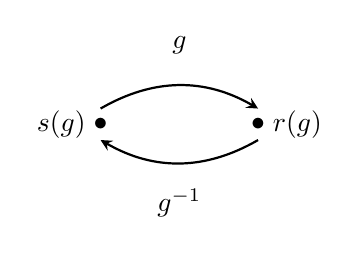
\begin{tikzpicture}
\draw  (0,1) node {$g$};
\draw  (0,-1) node {$g^{-1}$};
\draw [>=stealth, ->, thick] (-1,0.2) to[bend left] (1,0.2);
\draw [>=stealth, ->,thick] (1,-0.2) to[bend left] (-1,-0.2);
\draw  (-1,0) node {$\bullet$};
\draw  (-1.5,0) node {$s(g)$};
\draw  (1,0) node {$\bullet$};
\draw  (1.5,0) node {$r(g)$};
\end{tikzpicture}\]

In our setting, all the spaces will be topological spaces and the maps will be continuous. We will even simplify greatly our life by only looking at second countable, locally compact, étale groupoids with compact base space. From now on, we will only say \textit{étale}, forgetting about all other technical assumptions to gain in clarity.\\ 

Being étale means that the range map $r: G \rightarrow G^0$ is a local homeomorphism, i.e. for every $g\in G$, there exists a neighborhood $U$ of $g$ such that $r_{|U}$ is a homeomorphism. This implies in particular that every fiber $G^x = r^{-1}(x)$ and $G_x = s^{-1}(x)$ are discrete. When the base space $G^0$ has the additional property of being totally disconnected, we will say that $G$ is \textit{ample}. Here is a list of examples of étale groupoids.\\

\begin{itemize}
\item[$\bullet$] A (nice) compact space $X$ defines a trivial groupoid $G=G^0=X$ and source and target are the identity; in the opposite direction if the base space is a point, the groupoid is a group. One can already see how the notion of groupoid generalises both spaces and groups as promised.  \\

\item[$\bullet$] As an intermediate situation between these two cases, consider a discrete group $\Gamma$ acting by homeomorphisms on a compact space $X$. Define the \textit{action groupoid} as follow. Topologically, it is the space $G= X\times \Gamma \rightrightarrows G^0 = X$. The multiplication encodes the action
\[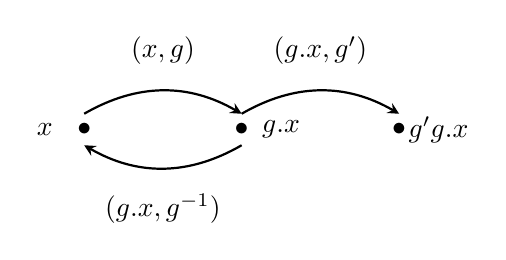
\begin{tikzpicture}
\draw  (0,1) node {$(x,g)$};
\draw  (0,-1) node {$(g.x,g^{-1})$};
\draw  (2,1) node {$(g.x,g')$};
\draw [>=stealth, ->, thick] (-1,0.2) to[bend left] (1,0.2);
\draw [>=stealth, ->,thick] (1,-0.2) to[bend left] (-1,-0.2);
\draw [>=stealth, ->, thick] (1,0.2) to[bend left] (3,0.2);
\draw  (-1,0) node {$\bullet$};
\draw  (-1.5,0) node {$x$};
\draw  (1,0) node {$\bullet$};
\draw  (1.5,0) node {$g.x$};
\draw  (3,0) node {$\bullet$};
\draw  (3.5,0) node {$g'g.x$};
\end{tikzpicture}\]
and this picture gives every element to reconstruct the groupoid.\\

\item[$\bullet$] If $R\subseteq X\times X $ is an equivalence relation, then $R$ as a canonical structure of groupoid with the base space being the diagonal $R^0 = \{ (x,x) \ | \ x\in X\}$ and the multiplication being the only one possible
\[(x,y)(y,z) = (x,z).\] 

\item[$\bullet$] More interesting is the \textit{coarse groupoid} $G(X)$ associated to a discrete countable metric space $(X,d)$ with bounded geometry, that is
\[\sup_{x\in X} |B(x,R)| < \infty \quad \forall R>0.\]
A nice way of thinking about this condition is to imagine yourself looking at the space with a magnifying glass of prescribed radius, but as great as you wish. Then you should not observe more and more points in your sight as you move around. In other words, the points fitting in the radius of your glass is uniformly bounded.\\

Now consider the $R$-diagonals:
\[\Delta_R = \{(x,y) \ | \ d(x,y) < \infty\}\subseteq X\times X\]
and take their closure $\overline{\Delta_R }$ in $\beta (X\times X) $ ($\beta Y$ being the Stone-\v{C}ech compactification of $Y$). The coarse groupoid is defined topologically as 
\[G(X) = \cup_{R>0} \overline{\Delta_R} \rightrightarrows \beta X ,\]
and is endowed with the structure of an \textit{ample} groupoid which extend the groupoid $X\times X \rightrightarrows X$ associated with the coarsest equivalence relation on $X$. The topological property of this groupoid encodes the metric or \textit{coarse} property of the space. For instance, $X$ has property A iff $G(X)$ is amenable, $X$ is coarsely embeddable into a Hilbert space iff $G(X)$ has Haagerup's property, etc.\\
\item[$\bullet$] The last construction is associated to what is often referred as an \textit{approximated group}, which is the data of $\mathcal N = \{ \Gamma , \{N_k\}\}$ where $\Gamma$ is a discrete group, and the $N_k$'s are a tower of finite index normal subgroups with trivial intersection, i.e. 
\[N_1 \triangleleft N_2 \triangleleft ... \quad \text{s.t. } \cap_k N_k = \{ e_\Gamma\} \text{ and } [\Gamma	: N_k] < \infty.  \]
Then the $\Gamma_k$'s are finite groups. Set $\Gamma_\infty = \Gamma$ for convenience (which is not usually finite!). For any discrete group $\Lambda$, there exists a left-invariant proper metric, which is unique up to coarse equivalence (take any word metric if the group is finitely generated). Let us denote by $|\Lambda |$ the coarse class thus obtained. Then the first object of interest in that case is the coarse space $X_\mathcal{N}$ defined as the \textit{coarse disjoint union}
\[X_\mathcal{N} = \coprod_k |\Gamma_k |.\]
Here the metric is such that $d(| \Gamma_i| , |\Gamma_j| )\rightarrow \infty $ as $i+j$ goes to $\infty$, $i\neq j$.\\

The second interesting object attached to $\mathcal{N}$ is the HLS (after Higson-Lafforgue-Skandalis \cite{HLS}, where it was first defined to build counter-examples to the Baum-Connes conjecture) groupoid. The base space is the Alexandrov compactification  of the integers 
\[G_\mathcal{N}^0 = \overline{\N},\]
and $G_\mathcal{N}$ is a bundle of groups with the fiber of $k$ being $\Gamma_k$. The topology is taken to be discrete over the finite base points, and a basis of neighborhood of $(\infty,\gamma)$ is given by 
\[\mathcal{V}_{\gamma, N} = \{(k, q_k(\gamma)) \ | \ k\geq N \} \quad N\in\N ,\]
where $q_k : \Gamma \rightarrow \Gamma_k$ is the quotient map.\\
 \end{itemize}

One of the reasons we use groupoids is that they are convenient to build interesting $C^*$-algebras. To see their relevance, one may start with the question \textit{What are operator algebraists doing?} A possible answer is that part of Noncommutative Geometry and Operator Algebras are devoted to the construction of interesting classes of $C^*$-algebras. For instance, \textit{nuclearity} was naturally introduced after Grothendieck's work, followed by a $C^*$-algebraic formulation. Arises then the question \textit{does there exist nonnuclear $C^*$-algebras?} A now classical result states that, when $\Gamma$ is a discrete group, the reduced $C_r^*(\Gamma)$ is nuclear iff $\Gamma$ is amenable. Calling out a nonamenable group, like any nonabelian free group, produces then a nonnuclear $C^*$-algebra. This game revealed itself to be very fruitful: study a property in some field and try to apply it to $C^*$-algebras to see what exotic being can be built out of it. The most common fields that have natural $C^*$-algbras associated to them are traditionally group theory, coarse geometry and dynamical systems (there are others like foliations etc, but let me just limit myself to these ones). This can be summarized in the following diagram.

%%%%%%%%%%%%%%%%%%%%%%%%%%%%%%%%%%%%%%%%%%%%%%%%%%%%%%%%%%%%%%%%%%%%%%%%%%%
\[\begin{tikzpicture}[node distance=1cm, auto,]
 %nodes
\node[punkt] (C) {$C^*$-algebras};\\
\node[punkt, above=of C] (G) {Groupoids};
\node[above=of G] (dummy) {};
\node[punkt, right=of dummy] (CG) {Coarse Geometry}
	edge[pil, bend left=45] node[auto] {$G(X)$} (G.east); 
\node[punkt, left=of dummy] (TD) {Topological dynamics}
	edge[pil, bend right=45] node[auto] [below left] {$\Omega\rtimes \Gamma$} (G.west); 
\node[punkt, above=of dummy] (GT) {Group theory}
	edge[pil, bend left=45] node[auto] {$Cay(\Gamma,S)$} (CG.north) 
	edge[pil, bend right=45] node[auto] [above left] {$\Gamma \curvearrowright \Omega$} (TD.north);

\draw[vecArrow] (G) to (C);
\end{tikzpicture}\]
%%%%%%%%%%%%%%%%%%%%%%%%%%%%%%%%%%%%%%%%%%%%%%%%%%%%%%%%%%%%%%%%%%%%%%%%%%%

Another interesting strategy is to try and translate a property in one of those upper boxes directly in terms of groupoids. Then the property can either be used to build $C^*$-algebras, either give a new definition in the case of other upper boxes. For instance, that is what we tried to do with Rufus Willett in our work on property T. Property T is originally a group property defined in terms of its unitary representations. In \cite{WillettYu}, Willett and Yu defined a geometric property T for monogenic discrete metric spaces with bounded geometry. Following their work, our first goal was to try and define a property T for (nice enough) topological groupoids so that in the case of groups and coarse groupoids, it reduces to these notions of property T. It gives then a notion of property T for dynamical systems, by considering property T for the action groupoid $X\rtimes \Gamma$. The second part of the work is dedicated to go down the last arrow, that is studying implications of property T for $G$ to its reduced and maximal $C^*$-algebras, and even more general completions of $C_c(G)$.\\

Let us first recall what is property T for discrete groups.\\

If $\pi : \Gamma \rightarrow B(H)$ is a unitary representation of $\Gamma$ on a separable Hilbert space, say that $\pi$ almost has invariant vectors if for every pair $(F,\varepsilon)$ where $F$ is a finite subset of the group and $\varepsilon$ a positive number, there exists a unit vector $\xi\in H$ such that 
\[ \| s.\xi - \xi \| < \varepsilon\quad \forall s\in F. \]
\begin{definition}
A group $\Gamma$ has property T if every representation that almost has invariant vectors admits a nonzero invariant vector.
\end{definition}

This definition is not the original one. Indeed property T was defined by Kazhdan in order to prove that \textit{some} lattices in \textit{some} Lie groups were finitely generated. It seemed a very specific property and application, but it turned out that property T gave very nice applications. Here are some of the most spectacular the author is aware of.\\

\begin{itemize}
\item[$\bullet$] Margulis supperrigidity theorem (about this, see Monod's \cite{MonodSuperrigidity} beautiful generalization, which Erik called the most beautiful paper he ever read);\\
\item[$\bullet$] existence of expander: for any infinite approximated group (in the sense of the examples above) $\Gamma$, the space $X_\mathcal{N}$ is an expander;\\
\item[$\bullet$] existence of Kazdhan projections which are very wild objects one should only approach with care; \\
\item[$\bullet$] more generally, property T was for a long time an obstruction to the Baum-Connes conjecture, up until the work of Lafforgue (\cite{LafforgueHyperbolic}, \cite{Lafforgue}). It still gives interesting properties for diverse crossed-product constructions as we will see.\\ 
\end{itemize}

One can prove easily that finite groups have T. Indeed, in that case, take the finite subset to be the whole group and look intensely at the identity
\[ \| s.\xi - \xi \|^2 = 2 ( 1 - Re \langle s.\xi ,\xi \rangle ).  \]
If $\xi$ is $(\Gamma,\varepsilon)$-invariant for $\varepsilon$ sufficiently small, then the above identity implies that $\frac{1}{|\Gamma |} \sum_{s\in \Gamma} s.\xi $ is nonzero because its inner-product with $\xi$ will have real part close to $1$. But $\xi$ is invariant.\\

Now take $\Gamma = \Z$ and look at the left-regular representation, i.e. $H = l^2\Gamma$ and 
\[(s.\xi)(x) = \xi(s^{-1}x).\]
Then if $\xi_n = \frac{1}{|F_n|} \chi_{F_n}\in H$ is the characteristic function of $F_n$ normalized to be a unit vector, one can check that 
\[ \sup_{s\in F}\| s.\xi_n - \xi  \| \rightarrow 0 \text{ as }n\rightarrow \infty \]
so that the regular representation always almost has invariant vectors. But it never has nonzero invariant ones, so that $\Z$ does not have T. This proof actually works for every infinite amenable group. \\

The moral of this story is that if one wants to find infinite groups with property T, one has to look at nonamenable groups. Maybe $\mathbb F_2$ or $SL(2,\Z)$? Actually not: they both surject to $\Z$ which does not have T, and this is an obstruction to having T as is obvious from the definition.\\

Finding infinite groups with property T is actually a hard problem. Here are some examples, without any proofs since these would go out of scope for these notes.\\
\begin{itemize}
\item[$\bullet$] $SL(n,\R)$ and $SL(n,\Z)$ if $n\geq 3$;\\
\item[$\bullet$] $Sp(n,1)$ and its lattices, which gives examples of infinite hyperbolic (in the sense of Gromov) groups having property T;\\
\item[$\bullet$] $Aut(\mathbb{F}_5)$ and $Out(\mathbb{F}_5)$ by a recent result of Nowak and Ozawa \cite{NowakOzawa}. Their proof is interesting in that they use numerical computations to reach their result using a previous result of Ozawa \cite{OzawaT};\\
\item[$\bullet$] $SO(p,q)$ with $p> q \geq 2$ and $SO(p,p)$ with $p \geq 3$. More generally, any real Lie group with real rank at least two, and all their lattices. Also, any simple algebraic group over a local field of rank at least two have T.\\ 
\end{itemize} 

To define property T for groupoids, we need to choose what kind of representations we are looking at, and to decide what are the invariant vectors.\\

A representation will be a $*$-homomorphism $\pi : C_c(G)\rightarrow B(H)$. A vector $\xi\in H $ is called invariant if \[f.\xi = \Psi(f).\xi \quad \forall f\in C_c(G).\]
The subspace of invariant vectors is denoted by $H^\pi$ and its orthogonal complement, the space of coinvariants, is denoted by $H_\pi$.\\

Here $Psi$... Groups\\

Let $\mathcal{F}$ be a family of representations.
\begin{definition}
$G$ has property T if there exists a pair $(K,\varepsilon)$ where $K\subseteq G$ is compact and $\varepsilon>0$ such that, for every $\pi \in \mathcal{F}$, there exists $f\in C_K(G)$ such that $\| f\|_I \leq 1$ and 
\[\|f .\xi - \Psi (f).\xi \| < \varepsilon \| \xi\| \quad \forall \xi \in H_\pi. \]
\end{definition}
 
The first thing we did was to study what were the relationships between groupoid property T and other property T.\\

\begin{itemize}
\item[$\bullet$] if $G=\Gamma$ is a discrete group, $\Gamma$ has property T iff $G$ has property T (in the groupoid sense);\\
\item[$\bullet$] if $X$ is a coarsely geodesic metric space, then $X$ has geometric property T iff $G(X)$ has property T;\\
\item[$\bullet$] in the case of a topological action, $X\rtimes \Gamma$ has property T iff $\Gamma$ has T w.r.t. the family $\mathcal{F}_X$ of representations $\pi : \C[\Gamma]\rightarrow B(H) $ s.t. there exists a representation $\rho: C(X) \rightarrow B(H)$ such that $(\rho, \pi) $ is covariant. This hypothesis simplifies in the case where there exists a invariant ergodic probability measure on $X$; in that case property T for $X\rtimes \Gamma$ and for $\Gamma$ are equivalent;\\
\item[$\bullet$] in the case of an approximated group $\Gamma$, then $G_\mathcal{N}$ has property T iff $\Gamma$ has T. This may sound disappointing, but if one refines the result, one gets the nice following property: $\Gamma$ has property $\tau$ w.r.t. $\mathcal{N}$ iff $G_\mathcal{N}$ has T w.r.t. the family of representations that extend to the reduced $C^*$-algebra of $G$.\\
\end{itemize} 

The last part of the work is devoted to the existence of Kazdhan projections. Recall, if $\mathcal{F}
$ is a family of representations, $C^*_\mathcal{F}(G)$ is the $C^*$-algebra obtained as the completion of $C_c(G)$ w.r.t. the norm
\[\| a \|_\mathcal{F} = \sup_{\pi \in \mathcal{F}} \{ \| \pi(a) \|\}. \]
A Kazdhan projection $p\in C^*_\mathcal{F}(G)$ is a projection such that its image in any of the representations in $\mathcal{F}$ is the orthogonal projection on the invariant vectors.\\

\begin{thm}
Let $G$ be compactly generated. Then if $G$ has property T w.r.t. $\mathcal{F}$, there exists a Kazdhan projection $p\in C^*_\mathcal{F}(G)$. 
\end{thm}

This gives an obstruction to inner-exactness. Denote by $F$ the closed $G$-invariant subset 
\[\{x\in G^0 \ | \ G^x \text{ is infinite }\}\]
and $U$ its complement.\\

\begin{thm}
Let $G$ be compactly generated and with property T. If one can find a sequence of points $(x_i)_i\subset U$ such that, for every compact subset $K \subset G$, $K$ only intersects a finite number of orbits $G.x_i = r(s^{-1}(x_i))$, then $G$ is not inner-exact. In fact it is not $K$-inner-exact. in particular, at least one of the groupoids $G$, $G_{|U}$ or $G_{|U}$ does not satisfy the Baum-Connes conjecture.
\end{thm}

%%%%%%%%%%%%%%%%%%%%%%%%%%%%%%%%%%%%%%%%%%%%%%%%%%%%%%%%%%%%%%
\subsection{Kazdhan projections and failure of $K$-exactness}
%%%%%%%%%%%%%%%%%%%%%%%%%%%%%%%%%%%%%%%%%%%%%%%%%%%%%%%%%%%%%%%

For $K\subset G$, $C_K(G)$ denotes the continuous functions supported in $K$. 

\begin{thm}
Let $G$ be an \'etale groupoid whose reduced $C^*$-algebra contains a non trivial Kazdhan projection $p$. Suppose there exists an invariant probability measure on $G^0$ and that there exists an open subset $U\subset G^0$ not equal to $G^0$ containing a sequence of points $(x_i)$ such that:
\begin{itemize}
\item[$\bullet$] $x_i$ has finite orbit ($x_i \in G^0_{fin}$);
\item[$\bullet$] for every compact $K\subset U$, the orbits $Gx_i= r(G_{x_i})$ ultimately don't intersect $K	$;
\end{itemize}
then $C^*_r(G)$ is not $K$-exact.
\end{thm}

\begin{proof}
Denote by $M_i$ the finite dimensional $C^*$-algebra $B(l^2G_{x_i})$ and $\lambda_i : C^*_r(G) \rightarrow M_i $ the corresponding left regular representation. We will show that the sequence 
\[ \begin{tikzcd} 0 \arrow{r} & 
C^*_r(G)\otimes \oplus M_i \arrow{r} & C^*_r(G)\otimes \prod M_i  \arrow{r}{q} & C^*_r(G)\otimes \prod M_i / \oplus M_i  \arrow{r} & 
0 \end{tikzcd}\]
is not exact in $K$-theory. We shall call $q$ the last map in this diagram.\\

Define the following $*$-morphism 
\[\phi \left\{ \begin{array}{rcl}
C^*_r(G) & \rightarrow  & C^*_r(G) \otimes \left(\prod M_i\right) \\
x        & \mapsto& x\otimes (\lambda_i(x))_i \\
\end{array} \right.\]
Claim: the image of $\phi$ is contained in the kernel of $q$.\\

Let $x\in C_r^*(G)$ and $\epsilon>0$. Let $K\subset G$ be a compact subset and $a\in C_K(G)$ such that $\| x - a \|_r <\varepsilon$. Let $\phi_i$ be the $*$-homomorphism defined in the same fashion as $\phi$ only with the first $i$ components of $\phi(x)$ equated to zero. Denote by $\overline x$ the class of $x$ in $C^*_r(G)\otimes \prod M_i / \oplus M_i $. Then $\overline {\phi(x)} = \overline{\phi_i (x)}$. Also, as the orbits $G_{x_i}$ are ultimately disjoint, there is a $i_0$ such that $\lambda_i(a)=0$ and thus $\phi_i(a)= 0$ for all $i>i_0$. This ensures
\[ \|\overline{\phi(x)} \|  = \|\overline{\phi_{i}(x)}\| = \|\overline{\phi_{i}(x)}-\overline{\phi_{i}(a)}\| < \varepsilon \]
hence $\overline{\phi(x)}=0$.\\

Let $p\in C^*_r(G)$ the Kazdhan projection. Then $P=\phi(p)$ goes to zero in the right side of the sequence above. Let us show that its class in $K$-theory does not come form an element in $K_0(C^*_r(G)\otimes \oplus M_i )$.\\

The invariant probability measure on $G^0$ induces a trace $\tau$ on $C^*_r(G)$. Define $\tau_i$ to be the trace $\tau \otimes tr$ on $C^*(G)\otimes M_i$, where $tr$ is the normalized trace on $M_i$. It is easy to see that $\tau_n(P) = \tau(p)>0$. But if $z\in K_0(C^*_r(G)\otimes \oplus M_i)$, $\tau_n(z)$ is ultimatley zero. This implies that the non triviality of $P$ ensures the non $K$-exactness of the sequence above in $K$-theory.  

\end{proof}

This result gives interesting examples of non $K$-exact $C^*$-algebras:
\begin{itemize}
\item[$\bullet$] if $X$ is an expander, the coarse groupoid of $X$ satisfies the hypothesis above, so that the uniform Roe algebra $C^*_u(X)\cong C_r^*(G)$ is not $K$-exact; in particular, if $\Gamma$ contains an expander almost isometrically, its reduced errrrr no?   
\item[$\bullet$] if $\Gamma$ is a residually finite group with property $(\tau)$, then any HLS groupoid associated to an approximating sequence of $\Gamma$ satisfies the hypothesis above so that $C_r^*(G)$ is not $K$-exact.
\end{itemize} 

%%%%%%%%%%%%%%%%%%%%%%%%%%%%%%%%%%%%%%%%
\section{Classification and the UCT}
%%%%%%%%%%%%%%%%%%%%%%%%%%%%%%%%%%%%%%%%

For $A$ a simple unital $C^*$-algebra, the Elliot invariant is:
\[Ell(A) = \left( K_0(A), K_0(A)_+ , [1_A]_0 , K_1(A), T(A) , r_A : T(A) \rightarrow S(K_0(A)) \right) ,\]
here $T(A)$ is the trace space and $r_A$ the paring $r_A(\tau)([p]) = [\tau(p)]$.\\

\textbf{Elliot's conjecture:} Separable, simple, nuclear are classifiable by Elliot's invariants.

\begin{thm}
Separable, simple, unital, nuclear, $\mathcal Z$-stable, UCT algebras are classifiable by Elliot's invariants.
\end{thm}

An example of a classification theorem: Elliot's theorem,

\begin{thm}
Let $A$ and $B$ unital AF-algebras and \[\alpha : K_0(A) \rightarrow K_1(A)\]
a unital order isomorphism, i.e. \[\alpha(K_0(A)_+) \subseteq K_0(B)_+ \quad \text{and} \quad \alpha([1_A])=[1_B].\]
Then there exists a unital $*$-isomorphism $\phi; A\rightarrow B$ such that $\phi_*=\alpha$.
\end{thm}

\newpage
%%%%%%%%%%%%%%%%%%%%%%%%%%%%%
\section{$C^*$-simplicity}
%%%%%%%%%%%%%%%%%%%%%%%%%%%%%
\subsection{General introduction}

Let $\Gamma$ be a discrete group. We will recall two equivalence relations on the set(?) of unitary representations of $\Gamma$, which are group homomorphisms
\[\pi: \Gamma \rightarrow U(H_\pi) \]
where $U(H_\pi)$ stands for the unitary group of a complex Hilbert space $H_\pi$. We will refer to such a representation as $(\pi, H_\pi)$ or even just $\pi$ or $H_\pi$ if no confusion is possible.\\

Let $\pi$ and $\sigma$ be two representations of $\Gamma$.
\begin{itemize}
\item[$\bullet$] $\pi \backsimeq \sigma$ iff there exists a unitary $u : H_\pi \rightarrow H_\sigma$ such that
\[ u\pi_\gamma u^* =\sigma_\gamma \quad \forall \gamma \in \Gamma.\]
\item[$\bullet$] $\pi \approx \sigma$ iff there exists a sequence of unitaries $u_n : H_\pi \rightarrow H_\sigma$ such that
\[ \| u_n\pi_\gamma u_n^* - \sigma_\gamma \| \rightarrow 0\quad \forall \gamma\in \Gamma.\]
\end{itemize}

\textbf{Fact:} It turns out that for a lot of groups (e.g. finite, abelian, compact, simple Lie groups,...), these two notions coincide
\[ \pi \approx \sigma \quad \text{iff}\quad \pi \backsimeq \sigma \quad \text{for }\pi,\sigma \text{ irreducible}.\]
Let $\hat \Gamma$ be the collection of all representations of $\Gamma$. A very hard problem is to describe
\[\hat \Gamma / \approx.\]
It can be done sometimes, e.g. for $\Z$ the irreducible representations are given by the circle, and any representation decomposes more or less uniquely into these.\\

Let us recall that the (left) regular representation 
\[\lambda: \Gamma \rightarrow U(l^2\Gamma)\]
is defined by $\lambda_g(\delta_h) = \delta_{gh}$. The reduced $C^*$-algebra $C_r^*(\Gamma)$ is the closure under the operator norm of the image of the regular representation, i.e.
\[C^*_r(\Gamma) = \overline{span \{ \lambda_\gamma\}_{\gamma\in \Gamma}}.\]
A representation $\pi $ is tempered if it extends to a $*$-representation of $C^*_r(\Gamma)$. This happens iff the linear extension
\[\pi : \C[\Gamma]\rightarrow B(H_\pi)\]
satisfies $\|\pi(a)\| \leq \|\lambda(a)\|, \forall a\in \C[\Gamma]$.\\

\textbf{Fact:} All representations are tempered iff the group is amenable.\\

Another (very hard) problem is to describe 
\[\hat \Gamma_r / \approx .\]

\begin{definition}
$\Gamma$ is $C^*$-simple if $C^*_r(\Gamma)$ is simple, i.e. admits no proper two sided closed ideal.
\end{definition}

\begin{thm}[Voiculescu]
$\Gamma$ is $C^*$-simple iff $\hat \Gamma_r / \approx$ is a point.
\end{thm}

\textbf{Examples of $C^*$-simple groups:}
\begin{itemize}
\item[$\bullet$] Non abelian free groups;
\item[$\bullet$] Torsion free hyperbolic groups;
\item[$\bullet$] $PSL(n,\Z)$;
\item[$\bullet$] Thompson's group $V$.
\end{itemize}

\subsubsection{Non $C^*$-simple examples}

Recall that a group $\Gamma$ if the trivial representation 
\[1_\Gamma : \Gamma \rightarrow U(\C) = \mathbb S^1; \gamma \mapsto id = 1;\]
is tempered. As a consequence, non trivial amenable groups are not $C^*$-simple as $1 \approx \lambda$ ($dim (l^2\Gamma ) \neq 1 )$.\\

More generally if there exists an amenable normal subgroup $K \vartriangleleft \Gamma$, then the quasi regular representation
\[\lambda_{\Gamma / K} : \Gamma \rightarrow U (l^2(\Gamma / K)); \ \lambda_{\Gamma / K}(\gamma) (\delta_{xK}) = \delta_{\gamma x K}; \]
is tempered, hence if $K$ is not trivial, $\Gamma$ is not $C^*$-simple. In particular any semi-direct product $K \rtimes H$ with $K$ amenable and non trivial is not $C^*$-simple.\\

Amenability being stable by extensions and increasing unions, any group has a largest normal amenable subgroup $R \vartriangleleft \Gamma$ called the amenable radical. The previous discussion shows that if $\Gamma$ is $C^*$-simple, then $R= \{e\}$. The converse does not hold and was completely answered by Kennedy et al.

\subsubsection{How to prove $C^*$-simplicity?}

\'a la Powers \cite{Powers1975simplicity}.

\begin{definition}
A group $\Gamma$ is a \textit{Powers group} if for every finite subset $F\subset \Gamma$ there exists a partition
\[\Gamma = C \coprod D \]
and a finite number of elements $\gamma_1,...,\gamma_n\in \Gamma$ with 
\begin{itemize}
\item[$\bullet$] $\gamma C \cap C = \emptyset$ for every $\gamma in F$:
\item[$\bullet$] $\gamma_i D \cap \gamma_j D = \emptyset$ for every $i\neq j$.
\end{itemize}
\end{definition}  

\textbf{Examples:}
\begin{itemize}
\item[$\bullet$] The free group on two generators $\mathbb F_2$ (Powers \cite{Powers1975simplicity});
\item[$\bullet$] Many other examples using "North-South" type dynamics (De la Harpe, Bridson, Osin).
\end{itemize}

Let us write a few words about the technique Powers used. For $\mathbb F_2 = \langle a,b\rangle$, let 
\[\tau : C^*_r(\mathbb F_2) \rightarrow \C ; a \mapsto \langle \delta_e , a \delta_e \rangle\]
be the canonical tracial state. 

\begin{thm}[Powers \cite{Powers1975simplicity}]
For every $a\in C_r^*(\Gamma)$, 
\[\tau(x) = \lim \frac{1}{mn} \sum_{i=1,n \\ j= 1,m} \lambda_a^i \lambda_b^j x \lambda_b^{-j} \lambda_a^{-i}\]
\end{thm}

\begin{cor}
$\mathbb F_2$ is $C^*$-simple.
\end{cor}

\begin{proof}
Let $J \vartriangleleft C_r^*(\mathbb F_2)$ be an ideal. For $x\in C_r^*(\mathbb F_2) $ let $x_{mn}=\sum_{i=1,n \\ j= 1,m} \lambda_a^i \lambda_b^j x \lambda_b^{-j} \lambda_a^{-i} $. If $x\in J$ then $(x^* x )_{mn}\in J$ so $\tau(x^*x)1_{C_r^*(\mathbb F_2)} \in \overline{J}^{\| \ \|} $. If $J$ is not trivial, it contains a non zero element $x$, which forces $1_{C_r^*(\mathbb F_2)} \in J$ as $\tau(x^* x)>0$. This ensures that $J = C^*_r(\mathbb F_2)$ and we are done. 
\end{proof}

\begin{cor}
$C^*_r(\mathbb F_2)$ has a unique tracial state.
\end{cor}

\begin{proof}
Let $\tau'$ be a tracial state on $C^*_r(\mathbb F_2)$. Then for $x\in C^*_r(\mathbb F_2)$,
\[\tau'(x)= \tau'(x_{mn}) \rightarrow \tau'(\tau(x)1) = \tau(x)\tau'(1) = \tau(x).\]
\end{proof}

%%%%%%%%%%%%%%%%%%%%%%%%%%%%
\subsection{Definitions}
%%%%%%%%%%%%%%%%%%%%%%%%%%%%

We only consider discrete countable groups, usually denoted by $\Gamma$.

\begin{definition}
A group is said to be $C^*$-simple if its reduced $C^*$-algebra is simple, i.e. has no proper closed two sided ideals. 
\end{definition}

A motivation for the interest toward such a notion can be the following result of Murray and Von Neumman: the Von Neumman algebra $L(\Gamma)$ is simple (no proper weakly closed two sided ideals) iff it is a factor iff $\Gamma$ is ICC (infinite conjugacy classes, i.e. all non trivial conjugacy classes are infinite). Another one is that simplicity is one out of the 5 criteria (unital simple separable UCT with finite nuclear dimension) needed in the classification theorem obtained by Winter et. al.\\  

Recall that, given two unitary representations of $\Gamma$, we say that $\pi$ is weakly contained in $\sigma$ and write 
\[\pi < \sigma\]
if every positive type function associated to $\pi$ can be approximated uniformly on compact sets by finite sums of such things associated to $\sigma$. In other words, if for every $\xi \in H_\pi$, $F\subseteq \Gamma$ finite and every $\varepsilon >0$, there exists $ \eta_1, \eta_2, ... , \eta_k$ such that
\[ | \langle \pi(s)\xi, \xi\rangle - \sum_i \langle \sigma (s)\eta_i,\eta_i \rangle| < \varepsilon \quad \forall s\in F.\]

Remark: one can restricts to convex combinations of normalized positive type functions.\\ 

If $\pi < \sigma$, then the identity $\C [\Gamma] \rightarrow \C [\Gamma]$ extends to a surjective $*$-morphisms
\[C_\sigma^*(\Gamma) \rightarrow C_\pi^*(\Gamma).\]

Indeed, it suffices to show that for every $a\in \C [\Gamma]$, \[ \| \pi(a)\| \leq \| \sigma(a)\|. \]
As $\| \pi(a)\|^2 = \| \pi(a^*a)\|$, we can suppose $a$ positive. Then
\[\begin{split}
 \langle \pi(s)\xi, \xi\rangle  & \leq   \sum_i t_i \langle \sigma (s)\eta_i,\eta_i \rangle +\varepsilon \\
				& \leq \| \sigma(a)\|+ \varepsilon
\end{split}\]
hence $\| \pi(a)\| \leq \| \sigma(a)\| +\varepsilon$, and let just $\varepsilon $ go to zero.

\begin{definition}
A group $\Gamma$ is $C^*$-simple if its reduced $C^*$-algebra is simple (i.e. has no proper closed two sided ideal).
\end{definition}

\begin{thm}
If $\Gamma $ has a non trivial amenable normal subgroup, then it is not $C^*$-simple.
\end{thm}

\begin{dem}
Let $N$ be a normal amenable subgroup of $\Gamma$. Let $(F_k)$ be a sequence of Folner sets for $N$, and 
\[\xi_k =\frac{1}{|F_k|}\chi_{F_k}\in l^2(\Gamma)\]
Then
\[\langle \lambda_\Gamma(s)\xi_k, \xi_k\rangle = 2- \frac{|F_k \Delta sF_k |}{|F_k|} \]
wich is $0$ if $s\notin N$, and goes to $1$ as $n$ goes to infinity if $s\in N$. In other words
\[\langle \lambda_\Gamma(s)\xi_k, \xi_k\rangle \rightarrow \langle \lambda_{\Gamma/N}(s)\delta_{eN} , \delta_{eN} \rangle,\]
which shows that $\lambda_{\Gamma / N} < \lambda_\Gamma$. This gives us a surjective $*$-morphism 
\[\phi : C^*_r(\Gamma)\rightarrow C^*_{\Gamma/N}(\Gamma).\]

A faster way which still works out when the ambient group is only locally compact is to point out that, $N$ being amenable, 
\[1_N < \lambda_N,\]
ensures by induction 
\[Ind_N^\Gamma 1_N = \lambda_{\Gamma / N} < Ind_N^\Gamma \lambda_N= \lambda_{\Gamma }.\]

But if $n\in N$ is non trivial, $\lambda_{\Gamma}(n)$ is non trivial and sent to $\lambda_{\Gamma /N}(n) = 1$ via $\phi$, so that $Ker\ \phi$ is a proper ideal in $C^*_r(\Gamma)$.\\	
\qed	 
\end{dem}

After the talk, Erik Guentner suggested the following proof. It is even shorter and doesn't assume any knowledge about weak containment or induction of representations. It is a weakening of the following fact: when $\Gamma$ is amenable, the trivial representation $1_\Gamma : C^*_{max}(\Gamma)\rightarrow \C$ extends to the reduced $C^*$-algebra.\\

Indeed let $a\in \C [\Gamma]$ and $(F_n)$ be a sequence of Folner sets for the support of $a$. Define $\xi_n = \frac{1}{|F_n|^\frac{1}{2}} \chi_{F_n} \in l^2(\Gamma )$. Then, suppose $a$ is positive, and compute
\[\begin{split}
\langle a \xi_n , \xi_n \rangle & = \sum_{s\in \text{ supp }a} a_\gamma \frac{|F_n \cap sF_n|}{|F_n|} \\ 
				& \rightarrow \| a \|_{1_\Gamma}
\end{split}\]
so that $ \| a\|_r \leq \| a\|_{1_\Gamma} $.\\

Now if $N$ is a normal amenable subgroup of $\Gamma$...\\

We saw that $\mathbb F_2$ is $C^*$-simple, yet it has a copy of $\Z$ as an amenable subgroup (non normal), and a normal (non amenable) subgroup: the commutator subgroup, which is an infinite rank free group, $\langle [x,y ] : x,y \in \mathbb F_2\rangle = \mathbb F([a^n, b^m] ; n,m) $. Both conditions are necessary.\\

This result led to following (false) conjecture: a group is $C^*$-simple iff it has no non trivial amenable normal subgroups.\\

%%%%%%%%%%%%%%%%%%%%%%%%%%%%%%%%%%%%%%%
\subsection{Completely positive maps}
%%%%%%%%%%%%%%%%%%%%%%%%%%%%%%%%%%%%%%%

If $A$ and $B$ are $C^*$-algebra, then a linear map $\phi : A\rightarrow B$ is called completely positive if 
\[\phi^{(n)}(a) = (\phi(a_{ij}))_{ij} \geq 0 \quad \forall a \in M_n(A)_+.\]
Denote $CP(A,B)$ the normed vector space of completely positive maps form $A$ to $B$. $S(A)$ denotes the state space of $A$, endowed with the weak-$*$ topology (it's then a convex subspace of $A^*$, compact when $A$ is unital).\\

Then: \\
\begin{itemize}
\item[$\bullet$] $CP(C(X),C(Y)) \cong C(Y, P(X))$ via $\mu_y(f) = \Phi(f)(y)$; \\

\item[$\bullet$] $CP(A,C(Y)) \cong C(Y, S(A))$ via $\omega_y(f) = \Phi(a)(y)$;\\

\item[$\bullet$] What about $CP(C(X),B)$? Continuous sections on the continuous field of $C^*$-algebras $\bigoplus_{\omega\in S(B)} B(H_\omega)$.\\
\end{itemize}

%%%%%%%%%%%%%%%%%%%%%%%%%%%%%%%%%%%%%%%%%
\subsection{Injective $C^*$-algebras}
%%%%%%%%%%%%%%%%%%%%%%%%%%%%%%%%%%%%%%%%%

Recall that an abelian group $M$ is injective if, given any injective homomorphism of abelian group $A \hookrightarrow B$, any homomorphism $A\rightarrow M$ extends to a homomorphism $B\rightarrow M$. In words: any homomorphism into $M$ extends to super-objects. We will often use the following commutative diagram
\[\begin{tikzcd}
B \arrow[dotted]{dr}{\exists} &  \\
A \arrow[hook]{u} \arrow{r}& M \\
\end{tikzcd}\]
to represent this situation. We will now turn to a analog notion in the $C^*$-algebraic world.\\

\begin{definition}
A $C^*$-algebra $M$ is \textit{injective} if, given an inclusion of $C^*$-algebra $A\subset B$, any injective $*$-homomorphism $A\rightarrow M$ extends to $B$ by a contractive completely positive (CCP) map.
\[\begin{tikzcd}
B \arrow[dotted]{dr}{\exists \ ccp} &  \\
A \arrow[hook]{u} \arrow{r}& M \\
\end{tikzcd}\] 
Even if the straight arrow are here supposed to be $*$-homomorphism, Stinespring's dilation theorem ensures that we can suppose all the arrows to be only CCP maps. We will say that $M$ is $\Gamma$-injective if $\Gamma$ acts by automorphisms on all the $C^*$-algebras in the diagram, and all the arrows are $\Gamma$-equivariant.
\end{definition} 

We will define a particular class of compact spaces acted upon by $\Gamma$, called $\Gamma$-boundaries, and show that there exists a maximal $\Gamma$-boundary $\partial_F \Gamma$, called the \textit{Thurston boundary}. \\

The first \textbf{major goal} of this presentation is to show that $C(\partial_F \Gamma)$ is $\Gamma$-injective.

%%%%%%%%%%%%%%%%%%%%%%%%%%%%%%%%%%%%%%%%%%%%%%%%%%%%%%%%%%%%%%
\subsubsection{Description of commutative injective algebras}
%%%%%%%%%%%%%%%%%%%%%%%%%%%%%%%%%%%%%%%%%%%%%%%%%%%%%%%%%%%%%%

\begin{lem} If $M$ is injective and $S\subset M$, define
\[Ann_M(S) = \{ m\in M \ | \ sm = 0 \forall s \in S.\]
Then there exists a projection $p\in M$ satisfying $Ann_M(S) = pM$.
\end{lem}

\begin{proof}
This is true if $M=B(H)$ for some Hilbert space. In the general case, embed $M$ unitally in some $B(H)$. By injectivity of $M$, there exists a CCP map $E: B(H)\rightarrow M$ such that $E(m)=m, \forall m\in M$ so $M\subset dom(E)$ (multiplicative domain). There exists a projection $p\in B(H)$ with $Ann_{B(H)}(S)= p B(H)$ (take the projection on $\cap_{s\in S} Ker(s)$). If $s\in S$, 
\[sE(p) = E(sp)= 0 \text{ hence }E(p)\in Ann_{M}(S).\]
Moreover if $m\in Ann_M(S)\subset pB(H) $, $pm = m$ and
\[E(p)m = E(pm) =E(m)=m\]
so that for $m=E(p)$, we get $E(p)$ is a projection. This also proves that $E(p)Ann_M(S) =Ann_M(S)$. A slight fiddling ensures then that $Ann_M(S)=E(p)M$.
\end{proof}

\begin{cor}
Let $X$ be a compact Hausdorff space. If $C(X)$ is injective then $X$ is Stonean, i.e. $\overline U$ is open for every open subset $U\subset X$.
\end{cor}

\begin{proof}
Let $U\subset X$ be open, and $S=C_0(U)$. By the previous lemma, there exists a projection $p\in C(X)$ such that $Ann_{C(X)}(S) = p C(X)$. But $p$ cannot be anyone else than the characteristic function of $\overline{U}^c$ so that $1-p =\chi_{\overline U}$ is continuous and $\overline U$ is open.
\end{proof}

\textbf{Note:} Infinite compact Stonean spaces are not metrizable (not even second countable). Suppose the contrary and get a sequence $x_i \rightarrow x$ in $X$ and open sets $U_n = B(x_n,\varepsilon_n)$, with $\varepsilon_n$ such that $\overline U_n \cap \overline U_m = \emptyset $ for every $n\neq m$. Set $U= \cup_{n}  U_{2n}$, then $x\in \overline U$ ($\overline U$ is open) so $x_n \in \overline U$ for large $n$ but $x_n \notin \overline U $ for $n$ odd.

%%%%%%%%%%%%%%%%%%%%%%%%%%%%%%%%%%%
\subsection{Furstenburg boundary}
%%%%%%%%%%%%%%%%%%%%%%%%%%%%%%%%%%%

If $\Gamma$ is a discrete group acting on a compact Hausdorff space $X$ (we will just say that $X$ is a $\Gamma$-space), the space of probability measures $Prob(X)$ endowed with the weak-$*$ topology is homeomorphic to the state space $S(C(X))$ with the topology of simple convergence. We identify $X$ with a closed subspace of $Prob(X)$ with the help of the Dirac masses ( $X \hookrightarrow Prob(X) ; x \mapsto \delta_x$ is an embedding). Recall that the action can be extended to $Prob(X)$, which is then a $\Gamma$-space by Banach-Alaoglu's theorem.

\begin{definition} A $\Gamma$-space $X$ is:
\begin{itemize}
\item[$\bullet$] \textit{minimal} if the only $\Gamma$-invariant closed subset of $X$ are itself and $\emptyset$;
\item[$\bullet$] \textit{strongly proximal} if $\overline{\Gamma . \mu}^{weak-*}$ contains $\delta_x$ for some $x\in X$;
\item[$\bullet$] a $\Gamma$-boundary if it is minimal and strongly proximal
\[ X\subset \overline{\Gamma . \mu}^{weak-*}\quad \forall \mu \in Prob(X).\]
\end{itemize}
\end{definition}

\textbf{Example:} Let $SL(2,\Z)$ act on the projective line $\R P^1$ (the quotient of $\R^2\backslash \{0 \}$ by the group of dilations) given by 
\[\begin{pmatrix} a & b \\ c & d \end{pmatrix} \begin{pmatrix} x \\ y \end{pmatrix} = \begin{pmatrix} ax +b y \\ cx + dy \end{pmatrix}.\]
Most $g\in Sl(2,\Z)$ are acting hyperbolically (two distinct eigenspaces, one expansive one contractive). Take $\mu\in Prob(\R P^1)$, and a generic element $g\in SL(2,\Z)$. As $n$ goes to $\infty$,
\[g^n .\mu \rightarrow_{weak-*} \ \delta_{\text{Expanding eigenspace}}\]
unless $\mu(\{\text{contractive eigenspace}\})>0$, hence \[\{\delta_{\text{Expanding eigenspace}}\}_{g\in SL(2,\Z)} \subset \overline{\Gamma. \mu}^{wk-*}.\]
Exercise: the set of these is dense in $\R P^1\subset Prob(\R P^1)$. 

\begin{thm}[Furstenburg] There exists a $\Gamma$-boundary $\partial_F \Gamma$ (now called the Furstenburg boundary) such that for any $\Gamma$-boundary $X$ there exists a continuous $\Gamma$-equivariant surjection $\partial_F \Gamma \twoheadrightarrow X$.
\end{thm}

\begin{proof}
Let $\mathcal B$ be the class of all $\Gamma$-boundaries. It is non empty as it contains the point space. Take
\[Z = \prod_{Y\in \mathcal B} Y \]
which is compact by Tychonoff's theorem. Equip $Z$ by the diagonal $\Gamma$-action. 
\begin{itemize}
\item[$\bullet$] It is strongly proximal: for any $\mu \in Prob(Z)$, a diagonal argument gives a weak-$*$ convergent net $g_i .\mu \rightarrow \delta_z$ for some $z\in Z$.   
\item[$\bullet$] It is not minimal, but Zorn's lemma ensures the existence of a minimal closed $\Gamma$-invariant subset $\partial_F \Gamma$ of $Z$.  
\end{itemize}
We obtain the desired map as the composition of the inclusion $\partial_F \Gamma \hookrightarrow Z$ with the projection on the $X$-factor $Z \twoheadrightarrow X$.
\end{proof}

\begin{thm}[Kalantar-Kennedy] $C(\partial_F \Gamma)$ is $\Gamma$-injective.
\end{thm}

\begin{lem} There exists a bijective correspondence between the completely positive maps from $C(X)$ to $C(Y)$ and the continous maps from $Y$ to $Prob(X)$. The statement remains true if one asks for equivariance. \textbf{send to a previous section on CP maps}
\end{lem}

\begin{lem}[Furstenburg] Let $X$ and $Y$ be two $\Gamma$-boundaries. Then any $\Gamma$-equivariant map $X\rightarrow Prob(Y)$ has image in $Y$, i.e. any UCP map $C(X)\rightarrow C(Y)$ is a $*$-homomorphism! Moreover there is at most one such map.
\end{lem}

\begin{proof}
Take $\mu : X \rightarrow Prob(Y)$. The image $\mu(X)\subset Prob(Y)$ is a closed $\Gamma$-invariant subspace: by strong proximality of $Y$, there exists $y\in Y$ such that 
\[ \delta_y \in \overline{\Gamma . \mu_x}^{wk-*} \subset \mu(X).\]
By minimality of $Y$, $\overline{\Gamma . \mu_x}^{wk-*}\cap Y = Y$, By minimality of $X$, $\mu^{-1}(Y)= X$ i.e. $\mu(X)\subset Y $.\\

Let $\mu, \eta: X\rightarrow Prob(Y)$ be two such maps. Then $\frac{1}{2}\mu +\frac{1}{2}\eta$, $\mu$ and $\eta$ all take values in $Y$ so that they are all equal. 
\end{proof}  

\begin{cor}\label{Unicity}
Any equivariant UCP map $ C(\partial_F \Gamma)\rightarrow C(\partial_F \Gamma)$ is the identity.
\end{cor}

Recall that if $A$ is a unital $\Gamma$-algebra, its state space $S(A)$ is convex compact $\Gamma$-space.

\begin{prop}[Gleason] \label{Gleason}
Let $Z \subset S(A)$ be a $\Gamma$-invariant closed convex subspace, which is minimal w.r.t. these properties. (Such a thing exists by Zorn's lemma.) Then
\[\partial_{ex}Z = \{ \phi \in Z \ | \ \phi \text{ is not a non trivial convex combination of anything in } Z\}\]
is a $\Gamma$-boundary.
\end{prop}
 
\begin{figure}[ht]
\centering
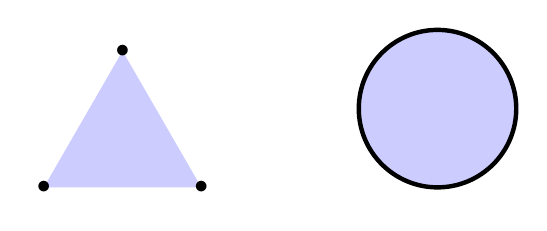
\begin{tikzpicture}[scale=2]

\draw [ultra thick, fill=blue!20] (2.5,0.5) circle (0.5);
    
\draw [ultra thick, draw=none, fill=blue!20]
       (0,0) -- (1,0) -- (0.5,0.866) -- cycle;
\draw  (0,0) node {$\bullet$};
\draw  (1,0) node {$\bullet$};
\draw  (0.5,0.866) node {$\bullet$};
\end{tikzpicture}
\caption{Two examples with $Z$ in blue and $\partial_{ex}Z $ in black.}
\end{figure}

\begin{proof}
There is a barycenter map $\beta : Prob(Z) \rightarrow Z$ such that 
\[\int_Z f d\mu = f(\beta(\mu)) \quad \forall f\in C(Z) \text{ affine}.\]
Indeed, if $\mu = \delta_z$, $\beta(\mu) = z$ and if $\mu = \sum \alpha_i \delta_{z_i}$ with $0\leq \alpha_i \leq 1$ and $\sum \alpha_i =1$, then $\beta(\mu) = \sum \alpha_i z_i$. Finite convex combinations are weak-$*$ dense in $Prob(Z)$ by the Hahn-Banach separation theorem. As $\beta$ is weak-$*$ continuous, and affine so uniformly weak-$*$ continuous, it extends to the whole space $Prob(Z)$.\\

Note: $\beta$ is $\Gamma$-equivariant continuous and satisfies $\beta(\mu)=z\in \partial_{ex} Z$ iff $\mu = \delta_z$.\\

Then, for any $\mu \in Prob(Z)$,
\[\beta(\overline{conv(\Gamma\mu)}) = \overline{conv (\Gamma \beta(\mu))}= Z,\]
the first equality coming from continuity, $\Gamma$-equivariance and affinity. Now, $\partial_{ex} Z$ is minimal, and if $\mu \in \partial_{ex} Z$, then 
\[A FINIR\]
\end{proof}

We are now ready for the main result of this section.\\

\begin{thm}[Kalantar-Kennedy]
$C(\partial_F \Gamma)$ is $\Gamma$-injective.
\end{thm}

\begin{proof}
First, observe that $l^\infty(\Gamma)$ is $\Gamma$-injective. Let indeed $A\subset B$ be an inclusion of $C^*$-algebras and $\phi: A \rightarrow l^\infty (\Gamma)$ a $*$-homomorphism. Then $ev_{e}\circ \phi$ is a state on $A$, so it extends to a state $\Psi$ on $B$. Define $\tilde \phi: B \rightarrow l^\infty (\Gamma)$ by 
\[\tilde \phi (b)(\gamma) = \Psi (\gamma^{-1}. b).\]
Then $\Psi$ is a UCP $\Gamma$-equivariant map that extends $\phi$.\\

Now, producing ucp equivariant maps
\[\begin{tikzcd} C(\partial_F \Gamma) \arrow{r}{\alpha} & l^\infty(\Gamma) \arrow{r}{\beta} & C(\partial_F \Gamma) \end{tikzcd} \] 
is sufficient to conclude, as their composition must be the identity by corollary \ref{Unicity}.\\

Define $\alpha : C(\partial_F \Gamma) \rightarrow l^\infty (\Gamma) $ by fixing $\mu\in Prob(\partial_F \Gamma)$ and set 
\[\alpha(f)(\gamma) = \mu (\gamma^{-1}.f).\]
By Gleason's theorem \ref{Gleason}, there is a $\Gamma$-boundary $X\subset S(l^\infty (\Gamma)) $. By universal property of $\partial_F \Gamma$, we have an equivariant surjection $\partial_F \Gamma \twoheadrightarrow X \subset S(l^\infty (\Gamma))$. By duality, we get a $\Gamma$-equivariant ucp map
\[\Psi : l^\infty (\Gamma) \rightarrow C(\partial_F \Gamma)\]
and we are done.
\end{proof}

As a final remark, one can point out that this last proof used the following useful fact: if $B$ is injective and $\phi: A \rightarrow B$ is a split injective $\Gamma$-ucp map, then $A$ is injective. We use this with $A=C(\partial_F \Gamma)$ and $B=l^\infty(\Gamma)$.  
%%%%%%%%%%%%%%%%%%%%%%%%%%%%%%%%%%%%%%%%%%%%%%%%%%%%%%%%%%%%%%
\subsection{Dynamical characterization of $C^*$-simplicity}
%%%%%%%%%%%%%%%%%%%%%%%%%%%%%%%%%%%%%%%%%%%%%%%%%%%%%%%%%%%%%%

(Facts we are using: \\ 
$C(\partial_F \Gamma)$ is $\Gamma$-injective, in particular any $\Gamma$-equivariant u.c.p. $C(\partial_f \Gamma)\rightarrow A$ is split, so is an isometric embedding,\\
$\partial_F \Gamma$ is totally disconnected, ) \\

The goal of this section is to prove the following theorem.

\begin{thm}
$\Gamma$ is $C^*$-simple iff the action of $\Gamma$ on $\partial_F \Gamma$ is free.
\end{thm}

Let's do first the forward direction.\\

Suppose the action is free. First, to show $C^*_r(\Gamma)$ is simple, it is enough to show that any representation 
\[\pi : C^*_r(\Gamma) \rightarrow B(H) \]
is injective. \\

By Arveson's extension theorem, $\pi$ extends to a u.c.p. map 
\[ \phi : C(\partial_F \Gamma)\rtimes_r \Gamma \rightarrow B(H). \]
Its restriction $\phi_0$ to $C(\partial_F \Gamma)$ is $\Gamma$-equivariant, because $C(\partial_F \Gamma)$ is in the multiplicative domain of $\phi_0$, and thus must be an isometric embedding, by $\Gamma$-injectivity of $C(\partial_F \Gamma)$ (it is split because $\C \subseteq B(H)$). The equivariant u.c.p. map $\phi_0$ is an isomorphism onto its image: extend its inverse form $im \  \phi_0$ to $im \ \phi$ and denote the resulting u.c.p map by $\tau$. \\

Claim: $\Psi = \tau \circ \phi $ is the canonical expectation $E : C(\partial_F \Gamma)\rtimes_r \Gamma \rightarrow C(\partial_F \Gamma)$ which is faithful. This implies $\pi$ is injective.\\

Let's end up with the claim. 
\begin{itemize}
\item[$\bullet$] $\Psi_{|C(\partial_F \Gamma)} = id_{C(\partial_F \Gamma)}$. Indeed, $\tau$ is the inverse of $\phi_0 = \phi_{C(\partial_F \Gamma)}$.
\item[$\bullet$] If $\gamma\neq e_\Gamma$, the action being free, for every $x$ there exists a function $f\in C(\partial_F \Gamma)$ such that 
\[f(x)\neq 0 \quad \text{and} \quad f(s^{-1}x) =0.\]
Now $C(\partial_F \Gamma)$ is in the multiplicative domain of $\Psi$, so
\[ \Psi(\lambda_s) f = \Psi( \lambda_s f) = \Psi( (sf)\lambda_s ) = (sf) \Psi( \lambda_s ) \]
which evaluated at $x$ gives $\Psi(\lambda_s)(x) = 0$, for all $x$, so $\Psi(\lambda_s)=0$. \\ 
\end{itemize}

The other direction is more intricated. It consists in two steps:\\
\begin{enumerate}
\item if $x\in \partial_F \Gamma$, then the stabilizer $\Gamma_x$ is amenable, which implies that $\lambda_{\Gamma/ \Gamma_x} <  \lambda_{\Gamma}$,\\
\item if $X$ is a $X$ is a $\Gamma$-boundary, and $\gamma\neq 0$ such that $int(X_s)\neq \emptyset$, then $\lambda_{\Gamma} \nless \lambda_{\Gamma/ \Gamma_x}  $, so that the kernel of $C^*_r(\Gamma)\rightarrow C^*_{\lambda_{\Gamma/ \Gamma_x}}(\Gamma)$ is a non trivial two sided closed ideal.\\
\end{enumerate}
This, together with the fact that $\partial_F\Gamma$ is topologically free iff it is free, concludes the proof.\\

First bullet: \\

\begin{itemize}
\item[$\bullet$] there exists a $\Gamma_x$-equivariant injective $*$-homomorphism
\[ \rho:  l^\infty (\Gamma_x ) \rightarrow l^\infty (\Gamma)\]
defined by $\rho(f)(ts_i)= f(t)$ for every $t\in\Gamma_x $, $\{s_i\}_i$ being a system of representatives of the right cosets $\Gamma_x \backslash \Gamma$.\\
\item[$\bullet$] there exists a $\Gamma_x$-equivariant u.c.p. map \[\psi : l^{\infty } \rightarrow C(\partial_F \Gamma),\] by universal property of $\partial_F \Gamma$, and the fact that the spectrum of $l^\infty(\Gamma)$ is $\beta \Gamma$. (for any compact $\Gamma$-space, there exists a $\Gamma$-map $\partial_F \Gamma \rightarrow P(X)$. take the dual of this map for $X = \beta \Gamma$).\\

\item[$\bullet$] The composition $\phi = ev_x \circ \psi \circ \rho$ defines a $\Gamma_x$-invariant state on $l^\infty(\Gamma_x)$, which concludes the proof.\\
\end{itemize}

Second bullet:\\

This needs a lemma:

\begin{lem} Let $X$ be a $\Gamma$-boundary.
For every non empty subset of $X$, every $\varepsilon >0$, there exists a finite subset $F\subset \Gamma \backslash \{e_\Gamma\}$ such that
\[ \min_{t\in F} \mu(tU^c) <\varepsilon \quad \forall \mu \in P(X).	 \]
\end{lem}

\begin{proof} 
Let $x\in U$. By strong proximality, there exists $t_\mu \neq e_\Gamma$ such that
\[\delta_x(U) - \mu(t_\mu U) = \mu(t_\mu U^c)<\varepsilon,\]
and by continuity of the action 
\[V_\mu = \{\nu\in P(X)\ | \ \nu(t_\mu U^c)< \varepsilon \}\]
is a neighboorhood of $\mu$. By compactness of $P(X)$ in the weak-$*$ topology, we can extract a finite cover such that 
\[P(X) = \cup_{i=1,m} V_{\mu_i}.\]
Then $F= \{ t_{\mu_1}, ..., t_{\mu_m}\}$ fills the requirements of the lemma.\\ 
\end{proof}

Suppose the action is not topologically free and let $s\neq e_\Gamma$ such that the interior $U$ of $X_s$ is not empty. Let $F$ the finite subset given by the lemma for $U$ and $\varepsilon = \frac{1}{3}$. Suppose 
\[\lambda_{\Gamma} < \lambda_{\Gamma / \Gamma_x}.\]
We will show this is absurd by looking at the coefficient $c_\gamma=\langle \lambda_\Gamma (\gamma)\delta_e , \delta_e \rangle$, which is $0$ unless $\gamma = e_\Gamma$.\\

On the finite subset $K= \{ tst^{-1} \}_{t\in F}$, approximate $c_\gamma$ up to $\varepsilon$ by a convex combination
\[ \sum_{j=1,n} \alpha_j \langle \lambda_{\Gamma / \Gamma_x} (\gamma)\xi_j , \xi_j \rangle\] 
of coefficients of the quasi regular representation.
Set 
\[\mu_j = \sum_{y \in \Gamma .x} |\xi_j(y)|^2 \delta_y \in P(X) \quad \text{and} \quad \mu = \sum \alpha_j \mu_j,\]
where we identify $\Gamma. x $ with $\Gamma / \Gamma_x$. \textbf{A FINIR}\\

\textbf{Questions:}\\
\begin{itemize}
\item[$\bullet$] Can we get a more direct proof for the last implication? (without representation theory) \\

\item[$\bullet$] It is not known in general wether the action of $\Gamma$ on $\partial_F \Gamma$ is amenable. If $X$ is a $\Gamma$-space such that one of the stabilizer is not amenble, the action cannot be amenable. Is it true that, if $\Gamma$ is exact, this is the only obstruction for the amenability of the action?
\end{itemize}

%%%%%%%%%%%%%%%%%%%%%%%%%%%%%
\subsection{Another proof}
%%%%%%%%%%%%%%%%%%%%%%%%%%%%%

The last subsection uses representation theory (induction) which makes one wonder if this could be avoided. While the implication 
\[\partial_F \Gamma \text{ is free } \Rightarrow	 \Gamma \text{ is }C^*\text{-simple}\]
is still good enough if one wants to stay clear of representation theoretic lingo, the other direction can be proven in another way.\\

This proof is taken from a set of notes that Ozawa wrote after giving lectures for the ``Annual Meeting of Operator Theory and Operator Algebras” at Tokyo university, 24–26 December 2014.\\

For $X$ a compact $\Gamma$-space and $H$ a subgroup of $\Gamma$, we denote by:\\

\begin{itemize}
\item[$\bullet$] $E_x : C(X)\rtimes_r \Gamma \rightarrow C^*_r(\Gamma)$ the canonical conditional expectation onto $C_r^*(\Gamma)$ given by extending the evaluation at $x$,   \\
\item[$\bullet$] $E_H : C^*_r(\Gamma) \rightarrow C^*_r(H)$ the canonical conditional expectation given by $E(\lambda_s) = \delta_{s\in H}$,\\
\item[$\bullet$] $\tau_H$ the canoncical trace $C^*_r(H) \rightarrow \C$.\\
\end{itemize} 

The first thing one can show is the following.

\begin{prop}
Let $X$ be a $\Gamma$-boundary, then 
\[C(X)\rtimes_r \Gamma\]
is simple.
\end{prop}

\begin{proof}
It is enough to show that any quotient map
\[\pi: C(X)\rtimes_r \Gamma \rightarrow B\]
is injective. By $C^*$-simplicity, $\pi$ restricts to an isomorphism on $C^*_{r}(\Gamma)$ so that the canoncial trace $\tau$ is well defined on $\pi(C_r^*(\Gamma)$. Seeing $\C$ as the sub-$C^*$-algebra of constant functions in $C(\partial_F \Gamma)$, we can extend $\tau$ to $B$.
\[\begin{tikzcd}
C(X)\rtimes_r \Gamma \arrow{r}{\pi}                     &                  B  \arrow[dotted]{rd}{\phi}                 &                                   \\
C^*_r(\Gamma) \arrow{r}{\cong}\arrow[hookrightarrow]{u} &  \pi(C^*_r(\Gamma)) \arrow{r}{\tau} \arrow[hookrightarrow]{u}& \C \subseteq C(\partial_F \Gamma) \\
\end{tikzcd}\]
Now $\phi \circ \pi $ restricts to a $\Gamma$-u.c.p. map $C(X)\rightarrow C(\partial_F \Gamma)$ which can only be the inclusion. This ensures that 
\[ C(X) \subseteq Dom(\phi \circ \pi). \]
As $\phi$ extends $\tau$, $\phi \circ \pi$ is the canonical conditional expectation $C(X)\rtimes_r \Gamma \rightarrow C(X)$ which is faithful. In particular, $\pi$ is faithful, and is injective.  
\end{proof}

Applying this to $X=\partial_F \Gamma$, we get that $C(\partial_F \Gamma)\rtimes_r \Gamma$ is simple. In that case, every stabilizer
\[\Gamma_x = \{ s\in \Gamma \ | \ sx=x \} \quad \forall x\in \partial_F\Gamma\]
is amenable. Moreover, the strong stabilizer
\[\Gamma^0_x = \{ s\in \Gamma \ | \ \exists U\text{ neighborhood of }x \text{ s.t. } s_U=id_U  \} \]
is a normal subgroup of $\Gamma_x$.(In particular, is is amenable.) In that case, we will apply the following proposition.

\begin{prop}
Let $X$ be a minimal compact $\Gamma$-space. If 
\[C(X)\rtimes_r \Gamma\]
is simple and there exists $x\in X$ such that $\Gamma^0_x$ is amenable, then $X$ is topologically free.
\end{prop}

\begin{proof}
By minimality, topological freeness is equivalent to $\Gamma^0_x=1$ for some $x$.\\ 

Indeed, if $\Gamma^0_x = 1$ for some $x$, every non trivial group element cannot fix any neighborhood of $x$ hence for every $s\neq e_\Gamma$, we get a sequence of points that converge to $x$ which are not fixed by $s$. By minimality,
\[X_s = \{ y \in X \ | \ sy \neq y \}\]
is a non empty dense open set of $X$ for every $s\neq e_\Gamma$. By Baire category's theorem, 
\[\cap_{s\in \Gamma\backslash \{e\}} X_s\]
is dense in $X$ so that $X$ is topologically free.\\

Let us show that $\Gamma^0_x=1$. Define a representation
\[\rho : C(X)\rtimes_r \Gamma \rightarrow B(l^2(\Gamma / \Gamma^0_x))\]
by $\rho(f\lambda_s) \delta_{\gamma \Gamma^0_x} = f(s\gamma.x) \delta_{s\gamma \Gamma^0_x}$. It is clearly covariant on the algebraic crossed-product.\\ 

To prove $\rho$ extends to the whole crossed-product, i.e. $\|\rho(a) \| \leq \| a\|_{C(X)\rtimes_r \Gamma}$, it is enough to show that 
\[\langle \ \rho(a)\delta_{\Gamma_x^0} , \delta_{\Gamma_x^0} \ \rangle \leq \| a\|_{C(X)\rtimes_r \Gamma}\]
because $\delta_{\Gamma^0_x}$ is cyclic. This follows from the fact that the latter is the composition $\tau \circ E_{\Gamma_x^0} \circ E_x$ of 3 u.c.p maps (so contractive).\\
 
Pick up $x$ such that $\Gamma^0_x$ is amenable and $s\in \Gamma$ arbitrary that fixes some neighborhood of $x$: there exists a neighborhood $U$ of $x$ such that $s_{|U}= id_{U}$. Let $f\in C(X)$ be nonzero and supported in $U$. Let us compute 
\[\rho(f\lambda_s)\delta_{\gamma\Gamma^0_x}.\]
\begin{itemize}
\item[$\bullet$] If $\gamma .x \in U$, then $s\gamma . x = \gamma . x$ and 
\[\rho(f\lambda_s)\delta_{\gamma\Gamma^0_x} = f(\gamma . x)\delta_{\gamma \Gamma^0_x} = \rho(f)\delta_{\gamma\Gamma^0_x}.\]  
\item[$\bullet$] If $\gamma .x \notin U$, $f(\gamma . x) = 0 = f( s \gamma . x)$, so that $\rho(f\lambda_s)\delta_{\gamma\Gamma^0_x} =\rho(f)\delta_{\gamma\Gamma^0_x}$.\\
\end{itemize}
This shows that $\rho(f (\lambda_s - 1)) = 0$. By injectivity, $\lambda_s = 1$ and $s=e_\Gamma$ hence $\Gamma^0_x=1$ and we are done.
\end{proof}

%%%%%%%%%%%%%%%%%%%%%%%%%%%%%%%%%%%%%%%%%%%%%%%%%%
\subsection{Thompson's group $V$ is $C^*$-simple}
%%%%%%%%%%%%%%%%%%%%%%%%%%%%%%%%%%%%%%%%%%%%%%%%%%

In this section, we prove that Thompson's group $V$ is $C^*$-simple. Recall that $V$ is defined as the group of piecewise linear bijections of $[0,1)$ with finitely many points of non differentiability, all of which are dyadic rational numbers. Such a function $f$ is entirely determined by two partitions 
\[[0, 1 ) = \coprod_{i=1}^n I_i = \coprod_{i=1}^n J_i\]
and a bijection $\begin{pmatrix} I_1 & ... & I_n \\ J_{\sigma(1)} & ... & J_{\sigma(n)}\end{pmatrix}$. The intervals $I_i$ and $J_i$ are of the type $[a,a+2^{-n})$, with $a$ dyadic rational in $[0,1)$. Then $f$ is defined on $I_i$ as the only linear increasing function applying $I_i$ to $J_{\sigma(i)}$.\\

\begin{figure}
\centering
\[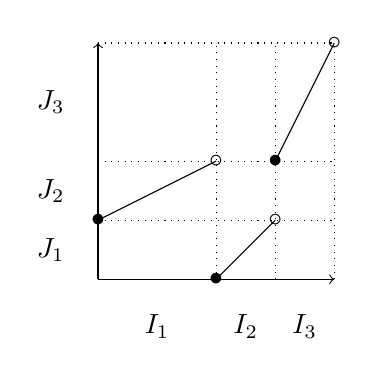
\begin{tikzpicture}[scale=3] 

\draw[->] (0,0) -- (0,1);
\draw[->] (0,0) -- (1,0);
\draw[dotted] (1,0) -- (1,1);
\draw[dotted] (0,1) -- (1,1);

\draw (0,0.25) -- (0.5,0.5);
\draw (0.5, 0) -- (0.75,0.25);
\draw (0.75,0.5) -- (1,1);

\draw[dotted] (0.5,0) -- (0.5,1);
\draw[dotted] (0.75,0) -- (0.75,1);
\draw[dotted] (0,0.25) -- (1,0.25);
\draw[dotted] (0,0.5) -- (1,0.5);

\draw (0,0.25) node {$\bullet$}; \draw (0.5,0.5) node {$\circ$};
\draw (0.5,0)  node {$\bullet$}; \draw (0.75,0.25) node {$\circ$};
\draw (0.75,0.5) node {$\bullet$}; \draw (1,1) node {$\circ$};

\draw (0.25,-0.2) node {$I_1$};
\draw (0.625,-0.2) node {$I_2$};
\draw (0.875,-0.2) node {$I_3$};
\draw (-0.2,0.125) node {$J_1$};
\draw (-0.2,0.375) node {$J_2$};
\draw (-0.2, 0.75) node {$J_3$};
\end{tikzpicture} \] 
\caption[]{The graph of $\begin{pmatrix} I_1 & I_2 & I_3 \\ J_2 & J_1 & J_3\end{pmatrix}$}
\end{figure}

In order to prove that $V$ is $C^*$-simple, we will:
\begin{itemize}
\item[$\bullet$] realize $V$ as a countable group of homeomorphisms of the Cantor set;
\item[$\bullet$] use the following result of Le Boudec and Matte-Bon (\cite{Boudec2016subgroup}, thm 3.7):
\begin{thm}
Let $X$ be a Hausdorff locally compact space and $\Gamma$ be a countable subgroup of $Homeo(X)$. Suppose that for every non empty open subset $U\subset X$, the rigid stabilizer
\[\Gamma_U = \{\gamma \in \Gamma \ |\  \gamma x = x \ \forall x\notin U\}\]
is non amenable. Then $\Gamma$ is $C^*$-simple.
\end{thm}
\end{itemize}

Let $G$ be an ample groupoid with compact base space. We also always suppsose that groupoids are second countable, Hausdorff and locally compact. Recall that a bisection $U\subset G$ is a set such that $s$ and $r$ are homoeomorphisms when restricted to $U$. In particular, any open bisection $U$ induces a partial homeomorphism
\[\alpha_U \left\{ \begin{array}{rcl}
s(U) & \rightarrow & r(U)\\ x & \mapsto & r\circ s_{|U}^{-1}(x)\\
 \end{array}\right.\] 
The topological full group $\llbracket  G \rrbracket$ is defined as the set of bisections $U$ of $G$ such that $s(U)=r(U)= G^0$. The operations are defined by 
\[e = G^0, \quad UV = \{gg' \ | \ g\in U , g'\in V  \text{ s.t. } s(g)=r(g')\}, \quad U^{-1}= \{g^{-1} \ | \ g\in U\}.\]

Recall that a Cantor space is any compact metrizable totally disconnected space without any isolated points. It is a standard fact that they are all homeomorphic. A model for $\Omega$ is the countable product $A^X$, where
\begin{itemize}
\item[$\bullet$] $A$ is a finite set, often reffered to as the \textit{alphabet};
\item[$\bullet$] $X$ is a countable set.
\end{itemize} 
Then elements of $\Omega$ are infinite words indexed by $X$. Denote by $\Omega_f$ the set of finite words \[\Omega_f =\coprod_{\text{finite } F\subset X} A^F,\]
then the topology on $\Omega$ is the one generated by the \textit{cylinders}
\[C_a = \{ w\in \Omega \ | \ w(x)= a(x) \ \forall x\in F=supp(a)\}.\]  
For finite words $a\in \Omega_f$, $l(a)$ denotes their length, and if $F=\N$, $x\in \Omega$, $ax$ denotes the concatenation of $a$ and $x$, i.e. the word obtained by first saying $a$ and then $x$.\\ 
 
\textbf{Examples:}
\begin{enumerate}
\item Let $\Gamma$ a countable discrete group acting on a Hausdorff compact space $X$ by homeomorphisms. Then $\llbracket X\rtimes \Gamma \rrbracket$ consists of the bisections of the type \[S=\coprod U_i\times \{\gamma_i\}\]
where $X = \coprod_{i=1}^n U_i = \coprod_{i=1}^n \gamma_i U_i$.\\
\item Let $\Z$ act on the Cantor space $\Omega= \{0,1\}^\Z$ by Bernoulli shift
\[ n (a_i)_i = (a_{i+n})_i\quad \forall n\in \Z , a \in \Omega.\]
Then $\llbracket \Omega\rtimes \Z \rrbracket$ consists of homeomorphisms $\phi : \Omega \rightarrow \Omega$ such that there exists a continuous function $n: \Omega \rightarrow \Z$ such that 
\[\phi(x) = n(x).x\quad \forall x\in \Omega.\]
\item Let $\Omega= \{0,1\}^\N$ be another model for the Cantor space. Define $T: \Omega \rightarrow \Omega$ continuous to be the shift
\[T(a_0, a_1,...)= (a_1,a_2,...).\]
Let $G_2$ be the so-called \textit{Cuntz} or \textit{Renault-Deaconu} groupoid defined by
\[\{(x,m-n,y)\ | \ x,y\in \Omega , m,n\in \N \text{ s.t. } T^mx= T^ny \}.\]
\textbf{Exercise:} The reduced $C^*$-algebra of $G_2$ is isomorphic to the Cuntz algebra
\[O_2 = C^* \langle s_1,s_2 \ | \ s_1 s_1^* + s_2 s_2^* =1 , s_1^*s_1 = s_2^*s_2 =1\rangle .\]
The open sets  
\[U_{a,b} = \{(ax,l(a)-l(b),bx)\ | \ x\in \Omega\}\]
define compact open bisections which cover $G_2$ when $a,b$ run across $\Omega_f$. \\

Then $\llbracket G_2 \rrbracket$ consists of the bisections of the type
\[S = \coprod_{i=1}^n U_{a_i,b_i}\]
where $\Omega = \coprod_{i=1,n} C_{a_i} = \coprod_{i=1,n} C_{b_i}$.\\

If for $a\in \Omega_f$, $I_a= [\overline a, \overline a + 2^{-l(a)})\subset [0,1)$, then 
\[\left\{\begin{array}{rcl}
\llbracket G_2 \rrbracket & \rightarrow & V \\
\coprod_{i=1}^n U_{a_i,b_i} & \mapsto & \begin{pmatrix} I_{a_1} & ... & I_{a_n} \\  I_{b	_1} & ... & I_{b_n} \end{pmatrix} \\
\end{array}\right.\]
is an isomorphism of groups.
\end{enumerate}

\begin{figure}[ht]
\centering
\[\begin{tikzpicture}[scale=3] 

\draw[->] (0,0) -- (0,1);
\draw[->] (0,0) -- (1,0);
\draw[dotted] (1,0) -- (1,1);
\draw[dotted] (0,1) -- (1,1);

\draw (0,0.25) -- (0.5,0.5);
\draw (0.5, 0) -- (0.75,0.25);
\draw (0.75,0.5) -- (1,1);

\draw[dotted] (0.5,0) -- (0.5,1);
\draw[dotted] (0.75,0) -- (0.75,1);
\draw[dotted] (0,0.25) -- (1,0.25);
\draw[dotted] (0,0.5) -- (1,0.5);

\draw (0,0.25) node {$\bullet$}; \draw (0.5,0.5) node {$\circ$};
\draw (0.5,0)  node {$\bullet$}; \draw (0.75,0.25) node {$\circ$};
\draw (0.75,0.5) node {$\bullet$}; \draw (1,1) node {$\circ$};
\draw (0.5,-0.5) node {$S=U_{0,01}\coprod U_{10,00} \coprod U_{11,1}$ corresponds to $\begin{pmatrix} I_0 & I_{10} & I_{11} \\ I_{00} & I_{01} & I_1\end{pmatrix}$} ;


\draw (0.25,-0.2) node {$I_{0}$};
\draw (0.625,-0.2) node {$I_{10}$};
\draw (0.875,-0.2) node {$I_{11}$};
\draw (-0.2,0.125) node {$I_{00}$};
\draw (-0.2,0.375) node {$I_{01}$};
\draw (-0.2, 0.75) node {$I_{1}$};
\end{tikzpicture} \] 
\caption{The isomorphism $\llbracket G_2 \rrbracket \cong V$}
\end{figure}

The last example realizes $V$ as a countable subgroup of homeomorphsims of $\Omega$. If $U=C_a$ is a cylinder for $a\in \Omega_f$, then the rigid stabilizer $V_U$ is isomorphic to $V$. But $V$ contains a nonabelian free groups, hence is nonamenable. The above theorem ensures that $V$ is thus $C^*$-simple.  \\

\newpage
%%%%%%%%%%%%%%%%%%%%%%%%%%%%%%%%%%%
\section{Weakly and non-weakly band dominated operators}

\subsection{Approximation of band dominated operators}

In the following, $X$ denotes a discrete metric space (e.g. $\Z$) with bounded geometry. This last requirement means that, for each positive number $r$, the cardinality of the $r$-balls is uniformly bounded, i.e. the number $N_r = \sup_{x\in X } |B(x,r)|$ is finite. For $T\in B(l^2 X)$, define the \textit{matrix coefficients} of $T$ by
\[T_{xy} = \langle \delta_x , T\delta_y \rangle \quad  \forall x,y\in X.\]
Think of $T$ as a matrix $(T_{xy})$ indexed by $X$. The propagation of such a $T$ will then be the (possibly infinite) number
\[prop(T) = \inf \{d(x,y) \ | \ T_{xy} \neq 0 \}. \]
If the propagation of $T$ is finite, we will say that $T$ is \textit{bounded} or has \textit{finite propagation}. \textit{Band dominated operators} are the norm limits of bounded operators. They form a $C^*$-algebra $C^*_u(X)$, called the \textit{uniform Roe algebra} of $X$.\\

\textbf{Questions:} 
\begin{enumerate}
\item If $T$ is band dominated, how can we approximate it by bounded operators?
\item How can we recognize when $T$ is band dominated?
\end{enumerate}

The two next numbers will give partial answers to these two questions. Or at least try to explain why they are not trivial.

\subsection{Approximation by bounded operators}

For $T\in B(l^2X)$ band dominated, define $T^{(n)}$ to be the operator with matrix coefficients
\[T^{(n)}_{xy} = \left\{ \begin{array}{lr} T_{xy} & \text{ if }d(x,y)\leq n  \\ 0 & \text{ otherwise. }\end{array}\right. \] 
We hope that $T^{n}$ converges to $T$ in norm as $n$ goes to $\infty$.\\

As an example, take $X= \Z$ with its canonical metric (given by the absolute value). Each $f\in C(\mathbb S^1)$ gives rise to a multiplication operator $M_f\in B(L^2(\mathbb S^1 ))$, and by Fourier transform to a convolution operator $T_f\in B(l^2\Z)$. It is the operator of norm $\| f\|_\infty$ with matrix coefficients $(T_f)_{xy}$ proportional to $\hat f(x-y)$.\\
In particular, if $f= \sum_{n=-N}^N \lambda_n z^n$ is a trigonometric polynomial, then $T_f$ is bounded as $\hat f(n) =0$ for $|n| >N$. This ensures that every $T_f$ is band dominated, as every continuous functions is a uniform limit of trigonometric polynomials. For such operators, our naive guess 
\[ `` \ T^{(n)}_f \rightarrow_{\| \|} T_f \text{ ''}\]
is equivalent to 
\[``\ \sum_{n=-N}^N \hat f(n)z^n \rightarrow_{\|\|_\infty} f \text{ ''}\]
which is false. It is even worse: one can have $\| T_f \| = 1$ while $\|  T_f^{(n)} \| $ goes to $\infty$ (Baire category argument, see \cite{stein2003princeton} p. 167) and this implies (by uniform boundedness theorem) that $(T_f^{(n)})_n$ does not even converges to $T_f$ in the strong operator topology.

\subsection{Weakly band dominated operators}

\begin{definition}
An operator $T\in B(l^2 X)$ has $(r,\varepsilon)$-propagation if for every subsets $A,B\subset X$ such that $d(A,B)>r$, \[\| \chi_A T\chi_B\| <\varepsilon .\]
$T$ is weakly band dominated if, for every $\varepsilon >0$, there is $r>0$ such that $T$ has $(r,\varepsilon)$-propagation.
\end{definition}

Note: Bounded implies weakly band dominated, therefore, weakly band dominated being a closed condition, band dominated implies weakly band dominated, as the intuition suggests. \\

\textbf{Question:} Does weakly bounded implies bounded?\\

This was claimed without proof for spaces with finite asymptotic dimension by J. Roe ca '97, and actually proved
\begin{itemize}
\item[$\bullet$] by Rabinovich-Roch-Silbermann in '00 for $X=\Z^n$ \cite{rabinovich2001band};
\item[$\bullet$] by \v{S}pakula-Tikuisis in '16 for finite asymptotic dimension (and a bit more, finite decomposition complexity spaces for the curious reader) \cite{spakula2017relative};
\item[$\bullet$] by \v{S}pakula-Zhang in '18 for spaces with property A \cite{spakula2018quasi}.
\end{itemize}
We have no counterexamples to this date (25 jan. 2019).

\begin{thm}[Folklore]
The following are equivalent:
\begin{enumerate}
\item $T$ is weakly band dominated;
\item for every $\varepsilon>0$, there exists $\delta>0$ such that if $f\in l^\infty(X)_1$ and $Lip(f)\leq \delta$ then $\| [T,f] \| <\varepsilon$.
\end{enumerate}
\end{thm}

\begin{proof}
Let us start with the reverse implication. Say $d(A,B)> r$, then there exists $f\in l^\infty(X)_1$ satisfying $0\leq f \leq 1$, $f_{|A}=1$, $f_{|B}=0$ and $Lip(f)\leq \frac{1}{r}$. Then $f\chi_A = \chi_A$ and $f\chi_B = 0$ so that 
\[\begin{split}
\chi_A T \chi_B & = \chi_A [f,T]\chi_B
\end{split}\] 
and $\| \chi_A T\chi_B \| \leq \frac{1}{r}$.\\

Remark: the function
\[f(x)= \max \{0, 1-\frac{d(x,A)}{r}\}\]
does the job. The Lipschitz constant is smaller than $\frac{1}{r}$ because of the easy inequality
\[ | d(x,A) - d(y,A) | \leq d(x,y) \quad \forall x,y \in X ,A \subset X. \] 
\end{proof}

\subsection{Characterizing membership in the Roe algebra}

The main goal of this section is to prove the following result, after the work of Spakula and Tikuisis.

\begin{thm}
Consider the following properties of an operator $b\in B(l^2 X)$.
\begin{enumerate}
\item $\lim \| [b , f_n] \| =0  $ for every very lipschitz sequence $(f_n) \subset C_b(X)$;
\item $b$ is quasi local;
\item $[b , g ] \in \mathfrak K( l^2X)$ for every Higson function $g\in C_h(X)$;
\item $b \in C^*_u(X)$. 
\end{enumerate} 
Then $(4) \implies (1) \iff (2) \iff (3) $. Moreover if $X$ has finite asymptotic dimension, then $(4)$ is equivalent to all of these.
\end{thm}

Some remarks are in order. 
\begin{itemize}
\item[$\bullet$] These results grew out of a question of John Roe, who asked about the implication $(2) \implies (4)$ when $X$ has \textit{finite asymptotic dimension} (FAD).
\item[$\bullet$] The theorem in \cite{spakula2017relative} is better: $(2)\implies (4)$ when $X$ has straight \textit{finite decomposition complexity} (FDC), which is much weaker than FAD. For instance, $\Z \wr \Z$ has FDC but not FAD, while FAD always implies FDC.
\item[$\bullet$] There is a follow up paper which shows $(2)\implies (4)$ when $X$ has property A, an even weaker condition. This last result will be treated in a following number.
\end{itemize}

Let us understand the conditions better.

\subsubsection*{Very Lipschitz condition} Recall that a function $f$ is Lipschitz if its Lipschitz modulus 
\[Lip(f) = \sup_{x\neq y} \frac{|f(x) - f(y)|}{d(x,y)}\]
is finite. More precisely, a function $f$ is $L$-Lipschitz if $Lip(f) \leq L \iff |f(x)-f(y)|\leq L d(x,y), \quad \forall x \neq y $.\\

A sequence $(f_n)\subset l^\infty (X)$ is \textit{very Lipschitz} if
\begin{itemize}
\item[$\bullet$] the sequence is uniformly bounded: $\exists C> 0 $ such that $\| f_n \| \leq C$;
\item[$\bullet$] $\lim Lip(f_n) = 0$.
\end{itemize} 
With this notation, the condition $(1)$ is equivalent to 
\[\forall \varepsilon > 0 , \exists L> 0 \text{ s.t. if } \|f \| \leq 1 \text{ and } Lip(f)\leq L \text{ then } \| [b,f] \| <\varepsilon. \]
Indeed, one direction is obvious, and suppose there exists $\varepsilon > 0 $ such that for every $L> 0$ there is a $f\in l^\infty (X)$ with $\| f\| \leq 1$, $Lip(f)\leq L $ and $\| [b, f ] \| \geq \varepsilon$. Take $L=\frac{1}{n}$ to get a very Lipschitz sequence $(f_n)$ with $\| [b,f]\| \geq \varepsilon > 0$, which contradicts $(1)$.\\

\subsubsection*{Quasi-locality} Recall that $b\in B(l^2X)$ is quasi-local iff $\forall \varepsilon> 0$, $b$ has finite $\varepsilon$-propagation,
iff $\forall \varepsilon > 0, \exists  r > 0$ such that $\forall f,g \in l^\infty (X)$, if $\|f\| , \|g\| \leq 1 $ and $d(supp(f), supp(g))\geq r$ then $\| fbg \| < \varepsilon$.\\

Let us introduce the space 
\[C_{L,\varepsilon} = \{ a \in B(l^2 X) \ : \ \| [a,f] \| < \varepsilon \quad \forall f\in l^\infty(X)_1 \text{ s.t. } Lip(f)\leq L \}.\]
What was said above reduces to the fact that the algebra of quasi-local operators is exactly
\[\bigcap_{\varepsilon > 0} \bigcup_{L>0} C_{L,\varepsilon}.\]

\subsubsection*{Higson functions} A function $g\in l^\infty (X)$ is said to be a Higson function, algebra denoted by $C_h(X)$ iff
$\forall \varepsilon > 0, \forall  r > 0$,  there exists a finite subset $F\subset X$ such that if $x,y \notin F$ and $d(x,y)\leq r$, 
then $|g(x)-g(y)|\leq \varepsilon$.

\subsubsection{Roe's question on conditions (2) and (4)}
$(4)\implies (2)$ is not difficult. In short, quasi-locality is a closed condition, which is obviously satisfied by finite propagation bounded operators. \\

\textit{Closed condition} If $\forall \delta> 0 $, there is a quasi-local operator $b'$ such that $\| b - b' \| < \delta $, then $b$ is quasi-local.\\

\textit{Finite propagation operators are quasi-local} If $\xi \in l^2(X)$ is finitely supported and $prop(b)\leq r$, then $supp( b\xi ) \subset N_r( supp(\xi))$, and so if $d(supp(f), supp(g))> r$, then $gbf = 0$.\\

$(4)\implies (1)$ is again not too hard. \\
Condition (1) is closed and is satisfied by finite propagation operators. This follows from elementary estimates and a calculation of the kernel of the commutator.
\begin{lem}
If $b\in B(l^2X)$ such that $|b(x,y)|\leq C$ and $prop(b)\leq r$, then $\| b \| \leq C N_r$
\end{lem}

\begin{lem} Let $b$ as above and $f\in l^\infty(X) $. The kernel of $[b,f]$ is 
\[[b,f](x,y) = b(x,y) (f(x)-f(y))).\]
\end{lem}

Now $(4)\implies (1)$ follows: if $prop(b)\leq r$, then \[prop([b,f]) \leq r \text{ and } | [b,f](x,y)| \leq C Lip(f)r\] so that also $\| [b,f] \| \leq C r N_r Lip(f)$. As for the lemmas, the first point reduces to:
\[\begin{split}
 |b\xi (x)|  & \leq \sum_{y\in B_r(x)} |b(x,y)|\ |\xi(y)| \\
	& \leq C N_r^\frac{1}{2} \| \xi_{|B_r(x)} \|_2 \quad\text{ by CBC}.\\
\implies \| b\xi \|_2^2 & = \sum_x |b\xi (x)|^2 \\
			& \leq \sum_x C^2 N_r \| \xi_{|B_r(x)} \|_2^2 \\
			& \leq \sum_x \sum_{y\in B_r(y)} C^2 N_r | \xi(y)|^2 \\
			& \leq C^2N_r^2 \|\xi \|^2_2 
\end{split}\]
The second point is a direct calculation.

\subsubsection*{$(1)\implies (2)$}
The key point is the following.

\begin{lem}
If $A,B\subset X$ such that $d(A,B)\geq r$, then there exists a function $\phi : X \rightarrow [0,1]$ such that 
\begin{itemize}
\item[$\bullet$] $\phi =1$ on $A$,
\item[$\bullet$] $\phi =0$ on $B$,
\item[$\bullet$] $Lip(\phi) \leq \frac{1}{r}$.
\end{itemize}
\end{lem} 
\begin{proof}
Let us show that it gives the claimed implication. Let $\varepsilon >0 $, condition $(1)$ gives a constant $L$. Put $r> L^{-1}$. If then $f,g\in l^\infty(X)_1$ such that $d(supp(f),supp(g))\geq r$ we have $f\phi=f$ and $g\phi=0$ so that 
\[\| fbg\| = \| f[\phi, b]g\| \leq \| [\phi,b]\| <\varepsilon .\]
As for the lemma, just take
\[\phi(x) = \max \{ 0, 1 -\frac{d(x,A)}{r}\}.\]
\end{proof}

\subsubsection*{$(2)\implies (1)$}
The key here idea is: if $f$ has a small Lipschitz constant, then it varies slowly so that its level sets are well separated.\\

Let $f\in l^\infty(X)$ such that $0\leq f \leq 1$ and $Lip(f)\leq L$, and put 
\[\begin{split}
A_i = &  \{x\ | \frac{i-1}{N} < f(x) \leq \frac{i}{N}\} \quad i=2,N \\ 
A_1 = & \{x \ |  0\leq f(x) \leq \frac{1}{N} \} \end{split} \] 
Then $f \sim \sum_{i=1}^N \frac{i}{N}A_i := g $ (actually $\| f-g\| \leq \frac{1}{N}$) and also 
\[ d(A_i,A_j)\geq \frac{1}{NL} \quad \text{ if } |i-j|\geq 2.\]
Also the $A_i$'s are disjoint and cover $X$. we will now estimate $\| [b,g] \| $. Let $\varepsilon>0$,
\[\begin{split}
\| [g,b] \| & = \| [ \sum_i \frac{i}{N} A_i , b] \| \\
		& = \| \left( \sum_i \frac{i}{N} A_i \right) \ b  \ \left(\sum_i  A_i \right)-  
				\left(\sum_i A_i \right) \ b \ \left(\sum_i \frac{i}{N} A_i \right) \| \\
		& = \| \sum_{i,j} ( \frac{i}{N} -\frac{j}{N}) A_i b A_j\| \\
		& \leq \| \sum_{|i-j| = 1} \frac{1}{N} A_i b A_j\| +\| \sum_{|i-j|\geq 2} (\frac{i}{N}-\frac{j}{N})A_i b A_j \| \\ 
\end{split}\]
Let us label the summands of this last line by I and II. By quasi-locality of $b$, we get a $r=r(\varepsilon)>0$, then for any choice of $N$, put $L= L(N,\varepsilon)$ such that $L< (rN)^{-1}$. Any such $f$ with $Lip(f)\leq L$ satisfies $d(A_i,A_j)> r$ so that $\| A_ifA_j \| < \varepsilon $ for each term in the second summand, so that 
\[ (II) \leq N^2 \varepsilon. \]
For $(I)$, the pairs $(i,j)$ can be split up into $4$ classes: ($i$ odd, $j = i+1$), ($i$ even, $j = i+1$) and the two symmetric cases. For each of these families, the sum is a block sum with orthogonal domain and range, hence the norm of the sum is less than the sup of the norm of the terms, so that 
\[(I) \leq \frac{4}{N}.\]
Let us wrap all of this up: if $\varepsilon$ is given, choose $N$ such that $\frac{4}{N} < \varepsilon$, choose $L= L(N,\frac{\varepsilon}{N^2})$. This gives:
\[\begin{split}
\| [b,g] \| & \leq (I) + (II) \\
	& \leq \frac{4}{N} + \frac{\varepsilon}{N^2} N^2 \\
	& \leq 2\varepsilon . \\
\end{split}\]   

\subsection{Heart of the paper}

Let us turn the attention to the most important result of the paper:
\[\text{If }X\text{ has FAD, then }(1)\implies (4).\]

\begin{thm}
Let $X$ be a bounded geometry uniformly discrete metric space. If $X$ has finite asymptotic dimension, then
\[\forall \varepsilon>0, \exists L>0 \text{ s.t. }a\in Commut(L,\varepsilon) \implies a \in C^*_u(X) \] 
and
\[ a\in Commut(L,\varepsilon) \iff \| [a,f] \| <\varepsilon \quad \forall f\in l^\infty(X)_1, Lip(f)< L.\]
\end{thm}

\subsubsection*{Review of asymptotic dimension}

Recall that $X$ has \textit{asymptotic dimension} less than $d$ if for every $r>0$, there exists a bounded cover $X$ which is $(d,r)$-separated. The typical example is the group $\Z$ with the metric induced by the absolute value, which has asymptotic dimension bounded by $1$. As an exercise, prove that $asdim(\Z^n) \leq n$.\\

In the context of $asdim \leq 1$, conditional expectations into block subalgebras are very natural. Consider subsets $\{U_i\}$ of $X$ which are pairwise disjoint and $u_i$ the correponding multiplication operators. Define 
\[\theta(a) = \sum_i u_i a u_i \quad \forall a \in B(l^2 X).\]
\begin{itemize}
\item[$\bullet$] $\theta(a)$ is SOT convergent;
\item[$\bullet$] $\theta$ is lower continuous;\\
Both of these follow essentially from
\[\begin{split}
\| \theta(a) \xi\|^2 & = \sum_i \| u_i a u_i \xi \|^2 \quad \text{by orthogonality of the support,} \\
			& \leq \| a \| \ \sum_i \| u_i \xi\|^2 \\
			& \leq \| a \| \ \| \xi\|^2  
\end{split}\]
Take the directed systems of all the sums over finite subsets of $I$, in which case the sum is finite.
\item[$\bullet$] $\theta$ is a conditional expectation. (Meaning it is CP, $\theta(xay)=x\theta(a)y$ when $x,y$ are block diagonals wrt $\bigoplus_i l^2U_i$, and $\theta(a)$ is block diagonal.)
\end{itemize}

Write $u=\sum_i u_i$. \\

\textbf{Fact:} if $prop(a)\leq r$ and $\mathcal U$ is $2r$-separated, then $uau=\theta(a)$.

\begin{proof}
If $\xi \in l^2 X$, $supp(u_i\xi)\subset U_i$, so that $supp(a u_i \xi ) \subset N_r(U_i)$ which is disjoint from $U_j$, $j\neq i$. Hence the cross terms $u_j a u_i \xi$ vanish. We get for finite sums \[\sum_{i,j \in F} u_i a u_j \xi =\sum_{i\in F} u_i a u_i \xi,\]
and the result follows by continuity. 
\end{proof}

\textbf{Consequence:} If $b\in C^*_u(X)$, for every $\varepsilon >0$, there exists $r>0$ such that if $\mathcal U$ is $r$-separated, then 
\[\| ubu -\theta(b)\| <\varepsilon.\]
This renders the next proposition natural.
\begin{prop}(Cor 4.3) 
If $a\in Commut(L,\varepsilon)$, with the notations above, if $\mathcal U $ is $\frac{2}{L}$-separated, then 
\[\| uau -\theta(a)\| <\varepsilon.\]
\end{prop}

Remark: if the theorem is true, then the above discussion shows that the result above must be true.\\

\begin{proof}(of the theorem, assuming the above proposition)
If $asdim(X)\leq 1$, fix a big $r>0$: we get a bounded cover $\mathcal Y$ which is $(1,r)$-separated, meaning
\[\mathcal Y = \mathcal U \cup \mathcal V\]
with $\mathcal U$ and $\mathcal V$ $r$-separated families. Then, if $a\in B(l^2X)$,
\[a = uau + uav + vau + vav.\]
we want to show that if $a\in Commut (L,\varepsilon)$ and $r>4L^{-1}$, then each term on the right is near a finite propagation operator. \\

\textit{Claim:} this is true for $uau$ and $vav$. \\

This follows from the proposition: $\mathcal U$ is $r>4L^{-1}> 2L^{-1}$-separated so that
\[ \| uau -\theta(a) \| \leq \varepsilon \]
and $\theta(a)$ is block diagonal w.r.t. a bounded family, it is thus of finite propagation (less than $\sup_{\mathcal U} diam (U)$).\\

\textit{Claim:} this is true for $uav$ and $vau$.\\

Let $\mathcal U'=N_{L^{-1}}(\mathcal U)$, same for $\mathcal V'$. Both are at least $2L^{-1}$-separated. We thus obtain $f=\sum f_i$ with $f_i$ $[0,1]$-valued, with value $1$ on $U_i$, $0$ on $N_{L^{-1}}(U_i)^c$ and $Lip(f_i)\leq L$. Similarly for $\mathcal V$, we get $g=\sum_j g_j$. Then $uf=u$ and $vg=v$. Put 
\[W_{ij} = N_{L^{-1}}(U_i)\cap N_{L^{-1}}(V_j) \quad , W = \coprod_{i,j} W_{ij}\]
which is at least $2L^{-1}$-separated. Similarly, build $w$ and $w_{ij}$. we then calculate:
\[\begin{split} 
uav  &= ufagv \\
	&= ugafv +u [f,a]gv + u [a,g]fv \\
\text{So } \| uav-ugafv \| 	& \leq 2\varepsilon \\
\end{split}\]   

but now, $ugafv \in Commut(L,\varepsilon)$, so that the proposition applies using the $\{W_{ij}\}$ which are $2L^{-1}$-separated:
\[\| wugafvw -\theta_w(ugafv) \| \leq \varepsilon.\]
But $ wugafvw= ugafv$ since $wug ug $ and $fvw = fv $ ($supp (fv)\subset W$ and $supp(ug)\subset W$). And $\theta_w(ugafv)$ is block diagonal with finite propagation.
\end{proof}

It remains to prove the proposition. 

\subsubsection*{Block diagonal symmetries}

\begin{lem}
If $a \in C_{L,\varepsilon}$ and $\mathcal U $ is a $\frac{2}{L}$-separated family of $X$ then
\[ \| [uau , \overline{u}] \| \\< \varepsilon \]
where $u =\sum u_i$ is our usual notation for the characteristic function of $\cup U_i$, and $\overline u$ is a \textit{block diagonal symmetry}, i.e. an operator of the type $\sum \epsilon_i u_i$, $\epsilon_i\in \{ -1, 1\}$.
\end{lem}

\begin{proof}
Extend each $u_i$ to a $[0,1]$-valued $L$-Lipschitz function, which is $1$ on $U_i$ and zero outside of $N_{L^{-1}}(U_i)$. Then the $f_i$ have disjoint support so that
\[\overline{f}=\sum_i \epsilon_i f_i \]
satisfies $Lip (\overline f )\leq L $, $\| f \| \leq 1$ and $\overline f u =\overline u$. But 
\[[uau , \overline u ] = u [a, \overline f ] u \]   
which has norm smaller than $\varepsilon$.
\end{proof}

The block diagonal symmetries form a topological group (with the SOT topology), isomorphic to $\prod_{\mathcal U} \Z_2$ endowed with the product topology. It is thus a totally disconnected compact group, and has a unique Haar probability measure $d\overline u$.

\begin{lem}
Let $Z \subset X$ and $b \in B(l^2 Z)$. If \[ \| [b, \overline u ] \| < \varepsilon \quad \forall \overline u \ \text{ block diagonal symmetry} \]
then $\| b - E(b) \| < \varepsilon$, where $E: B(l^2 Z) \rightarrow \bigoplus  l^\infty (U_i)$ is the canonical expectation onto the block diagonal. Furthermore,
\[E(b) = \int_G \ \overline u  b \overline u  \ d\overline u.\]
\end{lem}

\textit{Remark:} the example of the two point space is helpful to understand what is happening. Let say 
\[ \overline u =  \begin{pmatrix} \epsilon_1 &  0 \\ 0 & \epsilon_2\end{pmatrix} \quad \text{and} \quad b=  \begin{pmatrix} x &  y \\ z & w \end{pmatrix}\]
then a simple calculation shows 
\[ \begin{split} \begin{pmatrix} x &  0 \\ 0 & w \end{pmatrix} 
		& = \frac{1}{4}\sum_{\overline u \in G} \overline u b \overline u \\
   		& = \frac{1}{4} \left( 
 \begin{pmatrix} x &  y \\ z & w \end{pmatrix}+ \begin{pmatrix} x &  -y \\ -z & w \end{pmatrix}+  \begin{pmatrix} x &  y \\ z & w \end{pmatrix}+ \begin{pmatrix} x & - y \\ -z & w \end{pmatrix}
\right).
\end{split}\]

The estimate is easy: 
\[ \| E(b)-b \|   \leq \frac{1}{4} \sum \|  b \overline u - \overline u b\| < \varepsilon.\]

\begin{proof}
First check that on the group $G$, the $*$-SOT, SOT and pointwise convergence coincide. Since the norms are all smaller than $1$, we can consider finitely supported vectors, or even basis vectors. \\

Next the integral is understood in the weak sense, meaning that the assertion is 
\[\langle E(b) \xi, \eta \rangle = \int_G \langle \ \overline u b \overline u \ \xi , \eta \rangle \ d\overline u \quad \forall \xi, \eta \in l^2 X.\]
 Ignoring existence, check the following matrix coefficients
\[ \langle E(b)\delta_i, \delta_j \rangle = \left\{\begin{array}{lr} b_{ii} & \text{ if }i =j \\ 0 & \text{else.}\end{array}\right. \]
and 
\[\begin{split}
\int_G \ \langle \overline u b \overline u  \ \delta_i , \delta_j   \rangle  \ d \overline u & = \int_G \ \langle b \overline u \ \delta_i , \overline u \ \delta_j \rangle d\overline u \\ 
				& = (\int_G \ \epsilon_i \epsilon_j \ d\overline u ) \ b_{ij} .
\end{split}\] 
But \[ \int_G \ \epsilon_i \epsilon_j \ d\overline u = \mathbb P (\epsilon_i = \epsilon_j ) - \mathbb P (\epsilon_i \neq \epsilon_j)\]
which is $\frac{1}{2} - \frac{1}{2}=0$ if $i\neq j$, $1$ otherwise.
\end{proof}

Finally let's put all the lemmas together to get the proposition.

\begin{proof} 
Let $\mathcal U $ be a $\frac{2}{L}$-separated family and $a\in C_{L,\varepsilon}$. \\
The first lemma gives 
\[ \| [ uau \ , \overline u ] \| < \varepsilon \quad \forall \overline u \in G,\]
and now $uau \in B(l^2 Z)$ for $Z = \cup U_i$, so by the second lemma,
\[ \| uau - E(uau) \| < \varepsilon.\]
The canonical expectation $E(uau)$ is $\theta_{\mathcal U}(a)$, and this concludes the proof.
\end{proof}

%%%%%%%%%%%%%%%%%%%%%%%%%%%%%%%%%%%%55

\subsection{Property (A)}

The last part of the section is devoted to prove the assertion (quasi-locality implies locality) when $X$ has property (A).

\subsubsection*{Property (A) and its friends}
\textit{Motivation:} let $G$ be a countable discrete group with a bounded geometry left-invariant metric $d$. For each $A\subset X$ and every $r>0$, define the $r$-corona of $A$ to be the set
\[\partial_r A = \{x \in X \ | \ 0< d(x,A) \leq R\}.\]

Here is a possible definition of amenability.

\begin{definition}
The group $G$ is \textit{amenable} if for all $r,\varepsilon>0$, there exists a finite subset $A\subset X$ satisfying 
\[ | \partial_r A | < \varepsilon |A|.\] 
\end{definition}

\textit{Remark:} we don't suppose the group to be finitely generated. For instance $G= \bigoplus_\Z \Z$ with the metric $l(n) = \sum_i \ i |n_i|$ is not finitely generated, yet is of bounded geometry and amenable. If $G$ is finitely generated, one does not need to quantify over $r$ in the definition and can use $\partial A$ instead.\\

This definition of amenability makes perfect sense for any bounded geometry metric space. However, it is a bit silly, since for any bounded geometry space $X$, the space $X \cup \N$ is amenable. Indeed, given $r>0$, take $A_r = [r,r+N]\subset \N$. Then $\frac{| \partial_r A | }{|A| } = \frac{2r}{N+1}$ is very small for $N$ large. This definition of amenabilty is thus local (`` something nice happens somewhere") when we actually want to say something about the global structure of $X$.

\begin{definition}
The metric space $X$ is \textit{uniformly locally amenable}, abreviated $(ULA)_\mu$ after on, if for all $r,\varepsilon>0$, there exists $s>0$ such that for all probability measure $\mu \in Prob(X)$, there is a finite subset $A\subset X$ satisfying 
\[ diam(A)\leq s \quad \text{ and } \quad \mu( \partial_r A ) < \varepsilon \mu(A).\] 
\end{definition}

\textit{Remarks:}
\begin{itemize}
\item[$\bullet$] The strict inequality is important, otherwise take $A=\emptyset$.
\item[$\bullet$] The condition would be vacuous without the condition $diam (A) \leq s$, with $s$ uniform on all probability measures. Otherwise just take the uniform probability on $A$ for all $A$: the measure of the $r$-corona is $0$.  
\item[$\bullet$] $(ULA)_\mu$ is equivalent to property (A), see \cite{BNSWW}.
\item[$\bullet$] If $G$ is a group, then if $G$ is amenable, $G$ is $(ULA)_\mu$. The proof is left as an exercise for the reader.
\end{itemize}

More definitions.

\begin{definition} [\cite{dadarlat2007uniform}]
The metric space $X$ is \textit{exact} if for all $r,\varepsilon>0$, there exists $s>0$ and a partition of unity $\{\phi_i\}_i$ on $X$ such that
\begin{itemize}
\item[$\bullet$] if $d(x,y) < r$, then 
\[ \sum_{i\in I} |\phi_i(x) - \phi_i(y)| < \varepsilon ,\] 
\item[$\bullet$] $diam( supp(\phi_i)) \leq s$ for every $i\in I$.
\end{itemize}
\end{definition}

\begin{definition}[\cite{ChenTesseraWangYu}]
The metric space $X$ has the \textit{metric sparsification property}, abreviated $MSP$ after on, if for all $r,\varepsilon>0$, there exists $s>0$ such that for all $\mu \in Prob (X)$, there exists $\Omega \subset X$ such that
\begin{itemize}
\item[$\bullet$] $\mu (\Omega) \geq 1- \varepsilon$,  
\item[$\bullet$] $\Omega$ is a $r$-disjoint union of $s$-bounded sets.
\end{itemize}
\end{definition}

\begin{thm}[by everyone above]
Exact $\implies_{(1)}$ $(ULA)_\mu$ $\implies_{(2)}$ MSP $\implies_{(3)}$ $Exact$.
\end{thm}

The implication (3) is harder, see Sako \cite{sako2013property}. The proof is $C^*$-algebraic: can we find a direct proof?

\begin{proof}
(1) Given $r,\varepsilon> 0$, let $\mu \in Prob(X)$, and $\{\phi_i\}$ be as in the definition with 
\[ \sum_{i\in I} |\phi_i(x) - \phi_i(y)| < \frac{\varepsilon}{N_r}. \]
Hence for each fixed $x$, 
\[\sum_{y : d(x,y)\leq r} \sum_{i\in I} |\phi_i(x) - \phi_i(y)| < \varepsilon = \varepsilon \sum_i \phi_i(x).\]
As $\mu$ is a probability measure,
\[\sum_x \mu(x) \sum_{y : d(x,y)\leq r}\sum_{i\in I} |\phi_i(x) - \phi_i(y)| < \varepsilon \sum_x \mu(x) \sum_i \phi_i(x).\]
hence there exists an index $i_0$ such that
\[\sum_x \mu(x) \sum_{y : d(x,y)\leq r}|\phi(x) - \phi(y)| < \varepsilon \sum_x \mu(x) \phi(x).\]
with $\phi = \phi_{i_0}$. now write $\phi = \sum a_i \chi_{F_i}$ where $a_i > 0$ and $F_{i+1} \subset F_{i}$. All the $F_i$'s are in $supp(\phi)$ so their diameter is bounded above by $s$.
\[\begin{split} 
 \sum_x \mu(x) \sum_{y : d(x,y)\leq r}| \sum_k a_k(\chi_{F_k}(x) - \chi_{F_k}(y) ) | & < \varepsilon \sum_x \mu(x) \sum_k a_k \chi_{F_k}(x)\\
\sum_x \mu(x) \sum_{y : d(x,y)\leq r} \sum_k a_k | \chi_{F_k}(x) - \chi_{F_k}(y) |  & < \varepsilon \sum_x \mu(x) \sum_k a_k \chi_{F_k}(x).\\
\end{split}\]
Hence
\[\sum_x \mu(x) \sum_{y : d(x,y)\leq r} | \chi_{F_k}(x) - \chi_{F_k}(y) |   < \varepsilon \sum_x \mu(x) \chi_{F_k}(x) = \varepsilon \mu(F_k) \]
for some $k=k_0$, and for $x\in \partial_r F_{k_0}$,
\[\sum_{y : d(x,y)\leq r} | \chi_{F_k}(x) - \chi_{F_k}(y) | \leq 1 \leq \sum_{x\in \partial_r F_{k_0}} \mu(x)  = \mu (\partial_r F_{k_0}) .\]
Set $A= F_{k_0}$, then
\[\mu(\partial_r F_{k_0}) < \varepsilon \mu (A).\]
\end{proof}

\newpage
\subsubsection*{Quasi-locality and property (A)}

The main goal of this section is to provide a proof of $(1)\implies (4)$ in the case where $X$ has property (A). Let us fix some notations.\\

For $(X,d)$ a metric space, a partition of unity will be given by a pair $(\phi,\mathcal U)$ where $\mathcal U$ is a cover of $X$ and $\phi$ is a map
\[\phi: X \rightarrow l^2(\mathcal U)_{1,+}\quad,\]
such that $x\mapsto \phi_{U}(x)$ is supported in $U$ for every $U\in \mathcal U$. (The notation $l^2(\mathcal U)_{1,+}$ means positive elements of norm $1$.) If $\mathcal U = \{U_i\}_{i\in I}$, we will identify $l^2(\mathcal U)$ with $l^2(I)$. \\
 
The characterization of property (A) which we use is the following, obtained by Dadarlat and Guentner in \cite{dadarlat2007uniform}.

\begin{thm} 
A metric space $X$ is called \textit{exact} if, for every $r,\varepsilon>0$, there exists a partition of unity $\phi: X \rightarrow l^2(\mathcal U)$ such that $\mathcal U $ is uniformly bounded with finite multiplicity and 
\[d(x,y)\leq r \implies \| \phi(x) - \phi(y) \|_{2} \leq \varepsilon.\]
If $X$ is discrete and of bounded geometry, exactness and property (A) are equivalent.
\end{thm} 

We will also need to know that property (A) implies the metric sparsification property, which was proven in the last section.\\

The key idea of the proof relies on an approximation property of quasi-local operators: their norm can be approximated by finitely supported vectors. This means that if $b\in \bigcap_\varepsilon \bigcup_L C_{L,\varepsilon}$,
\[\| b \| = \sup_{\|v \| =1 \ , \ diam( supp(v))<\infty} \|bv\|. \]
This relies on the following lemma.

\begin{lem}[\cite{spakula2018quasi}, lemma 5.2]
For every $M,L,\varepsilon$, there exists $s>0$ such that, for every $b\in C_{L,\varepsilon}$ with $\| b \| \leq M$, there exists $v\in l^2(X)$ satisfying $\|v\| = 1$, $diam(supp(v)) <s$ and 
\[\| b v\| \geq \| b\| -\varepsilon.\] 
\end{lem}

\begin{proof}(of the result, using the lemma) 
Let $X$ discrete with bounded geometry and property (A), and say $b\in B(l^2 X)$ is quasi-local and fix $\varepsilon>0$. Then there is $L>0$ such that $b\in C_{L,\varepsilon}$ and, by the lemma, a $s>0$ such that $\| T \|$  can be approximated up to $\varepsilon$ by $s$-supported vectors for every $T\in C_{2\varepsilon, L}$ with $\| T\| \leq M$.\\

Choose a partition of unity $\phi$ with uniformly bounded support and 
\[ d(x,y)\leq s+\frac{1}{L} \implies \| \phi(x) - \phi(y) \| \leq \varepsilon.\]

Let us show that the norm of \[a= b-\sum_i \phi_i b \phi_i = \sum_i \phi_i [\phi_i , b] \]
is small enough.\\

The following computation shows that $a\in C_{2\varepsilon, L}$:
\[\begin{split}
\| [a,f]\|      & = \| [\sum_i \phi_i [\phi_i , b],f] \| 		\\
		& \leq \| \sum_i \phi_i [b,f] \phi_i \| + \| [b,f]\|    \\
		& \leq 2\varepsilon
\end{split}\]
where we used $\| \sum_i \phi_i [b,f] \phi_i - \phi[b,f] \phi\| < \varepsilon$. This follows from the fact that, if $e_j$ are positive contractions with $\frac{2}{L}$-separated support, and $T\in C_{\varepsilon,L}$, then $\| eTe-\sum_i e_i T e_i \| <\varepsilon $. This is not a trivial statement, and was proven in the last section (Cor 5.3 of \cite{spakula2018quasi}).\\

Of course, $\|a\| \leq 2M$, so we can apply the statement of the first paragraph to $a$: there exists a unit vector $v\in l^2X$ with support $F$ satisfying $diam(F) < s$ and $\| av \| \geq \|a\| -\varepsilon $, and 

\[\begin{split}
|\sum_{i} \phi_i(x) ( \phi_i(x)-\phi_i(y)) b_{xy}|   & \leq M (\sum_i \phi_i^2 (x) )^{\frac{1}{2}} \ (\sum_i |\phi_i (x) - \phi_i(y)|^2)^\frac{1}{2} \\
		& \leq M \|\phi(x) - \phi(y) \|_2 \\
\end{split}\]
so that if $x\in N_{L^{-1}}(F)$, $\|\phi(x) - \phi(y) \|_2 \leq \varepsilon$, and
\[\begin{split}
|av|_x  & = |\sum_{i, y\in F} \phi_i(x) ( \phi_i(x)-\phi_i(y)) b_{xy} v_y| \\
		& \leq \sum_{y\in F} |\sum_i\phi_i(x) ( \phi_i(x)-\phi_i(y)) b_{xy}| \ | v_y |\\
		& \leq \varepsilon M \sum_{ y\in F} | v_y |\\
		&  \leq \varepsilon M  N_{s}^{\frac{1}{2}}\  \| v \|.\\
\end{split}\]
Now $\| av \|^2 =  \sum_x |av|^2_x \leq  M^2  N_{s}^2  \| v \|^2 \varepsilon^2 +  \sum_{x\in N_{L^{-1}}} |av|^2_x$, but $a$ being in $C_{2\varepsilon, L}$, 
\[ \| \chi_{F} a \chi_{N_{L^{-1}}(F)}\| <\varepsilon \] hence $\| av \|^2 \leq (M^2  N_{s}^2 +1)^{\frac{1}{2}} \| v \| \varepsilon $.
\end{proof}

It remains to prove the lemma.

\begin{proof} 
Let $b\in C_{\varepsilon,L}$ and $M=\|b\|$. Let $v\in l^2(X)$ be a unit vector such that $\|bv \|  \leq \| b \| -\frac{\varepsilon}{2M}$ (so that $\|bw\| \geq \|bv\| -\varepsilon$). Denote by $\mu$ the probablity measure on $X$ defined by 
\[\mu(\{x\} ) = |v_x|^2 .\]
The MSP implies that there is a subset $\Omega \subset X$ with $\mu(\Omega^c)<\varepsilon$ and $\Omega$ is a $\frac{4}{L}$-separated disjoint union \[\Omega = \coprod_{\frac{4}{L}} \Omega_i\]
of uniformly bounded subsets, i.e. $diam(\Omega_i)<s$ for all $i$. Denote by $w_i = P_{\Omega_i}v$, and $w=\sum_i w_i$. Then the condition above says that $\|v-w \|^2 < \varepsilon$ and $diam(supp(w_i)) <s$ so if we could approximate $\| b\| $ using one of the $w_i$'s, that would end the proof.\\

There exists $f_i\in l^\infty(X)_1$ such that 
\begin{itemize}
\item[$\bullet$] $Lip(f_i)\leq L$,
\item[$\bullet$] $supp(f_i) \subset N_{L^{-1}}(\Omega_i)$,
\item[$\bullet$] $f_i = 1$ on $\Omega_i$ and $0$ outside of $N_{L^{-1}}(\Omega_i)$.
\end{itemize}
Then $f = \sum_i f_i$ and $1-f$ are also $L$-lipschitz functions and $fw=w$. But $bw = [b,f]w +fbw$ so
\[\begin{split} 
\| bw \|     & \leq  \varepsilon \|w\| + \| f b f w\| \\
 		& \leq 2\varepsilon \|w\| + \| \sum_i f_i b f_i w\| \\
\end{split}\]
In the last line, we used that $\| fbf - \sum f_i b f_i \| \leq \varepsilon$:\\

Now, the same trick $f_i b = [f_i,b] + bf_i$ entails that 
\[\begin{split} 
 \| \sum_i f_i b f_i w\|^2   & =  \sum_i \| f_i b w\|^2 \\
 		& \leq \varepsilon \sum_i \| w_i\|^2 +\sum_i \| b w_i\|^2   \\
		& \leq \varepsilon \| w\|^2 +\sum_i \| b w_i\|^2   \\
\end{split}\]
so that 
\[ (\| bw\| -3\varepsilon \| w \|)^2 \leq \sum_i \| b w_i\|^2 \leq \sum_i \frac{\| b w_i\|^2}{\| w_i\|^2}\|w_i \|^2 \leq \sup_i (\frac{\| b w_i\|^2}{\| w_i\|^2} )\|w\|^2 \]
from which follows that
\[\frac{\| bw\|}{\|w\| } \leq \sup_i\frac{\| b w_i\|}{\| w_i\|}+3\varepsilon.\]
and
\[ \sup_i\frac{\| b w_i\|}{\| w_i\|}+3\varepsilon \geq \frac{\|bv\| -\varepsilon \|v\| }{\|w\|}\geq \|bv\| -\varepsilon \geq \|b\| -2\varepsilon \]
so that there exists $i_0$ such that $\frac{\| bw_{i_0} \| }{\| w_{i_0} \| }\geq 6 \varepsilon,$ and $diam(supp(w_{i_0})) <s$. 
\end{proof}
%%%%%%%%%%%%%%%%%%%%%%%%
%%%%%%%%%%%%%%%%%%%%%%%

\newpage
\section{Haagerup}

\subsection{An example of a nonuclear $C^*$-algebra which has the MAP}

In his 1979 paper \cite{}, Haagerup showed that $C^*_r(\mathbb F_n)$ has the Metric Approximation property, this settling that CPAP and MAP are not equivalent. This paper is considered a landmark of the field, for several reasons. It contains several ideas that would bloom as properties of their own: Haagerup's property, Rapid Decay, etc.\\

The following statement can be extracted from the paper.

\begin{thm}
Let $G$ be a discrete group which has length $l$ of conditionally negative type. If $G$ has $(RD)_l$, then $C^*_r (G)$ has the MAP.
\end{thm}

Actually what is proven is that if $G$ has $(RD)_l$ w.r.t. a (CNT) length, then there exists a net of contrative bounded linear maps
\[T_\alpha : C^*_r (G) \rightarrow C^*_r (G)\]
which converges poinwise to the identity, i.e.
\[\lim_\alpha \|T_\alpha(x) - x\| = 0 \quad \forall x\in C_r^*(G).\]

You need to know how to build multipliers on the group $C^*$-algebra.
\begin{lem}
We say that $\phi: G \rightarrow \C$ is a \textit{multiplier} if there exists a unique bounded linear map $M_\phi :  C_r^*(G) \rightarrow  C_r^*(G)$ such that 
\[M_\phi(\lambda_s ) = \phi(s)\lambda_s\quad \forall s\in G.\]
If either one of these conditions is satisfied, then it is the case:
\begin{itemize}
\item[$\bullet$] $\phi$ is completely positive, and then $\| M_\phi\| = \phi(e)$;
\item[$\bullet$] $G$ has $(RD)$ with constants $C,\alpha$, and $K= \sup_{g} |\phi(g)|(1+|g|)^\alpha <\infty$. Then $\| M_\phi\|\leq CK$.
\end{itemize} 
In particular, finitely supported functions induce multipliers.
\end{lem}

Let's prove the statement.

\begin{proof}
Since free groups are metric trees, the length function is of (CNT) and, by Schonberg's theroem, 
\[\phi_t(g)=e^{-t|g|} \quad \forall t>0\]
are of (PT). \\

Define their restriction to the ball of radius $n>0$ and the error
\[\phi_{n,t}(g)=e^{-t|g|}1_{|g|\leq n}  \text{ and } r_t(g)=e^{-t|g|} \]
Both satisfy the second point of the lemma, $\phi_{n,t}$ is finitely supported, and $e_{t,n}$ has 
\[K_n = \sup  \sup_{|g|> n } e^{-t|g|}(1+|g|)^\alpha \rightarrow 0. \]
From this, it is standard to prove that up to renormalization, one can extract from the net $M_{\phi_{t,n}}$, which are of finite rank, a net which gives the MAP.
\end{proof}

The proof that $\mathbb F_n$ has (RD) is based on the estimate \[\|\lambda(a) \| \leq (k+1)\|a\|_2\]
if $a\in \C_{S_k}[G]$, then by Cauchy-Schwartz
\[\begin{split}
\|\lambda (a) \| & \leq \sum (k+1)\|a_k\|_2 \\
		& \leq (\sum \frac{1}{(1+k)^2} )^\frac{1}{2} \cdot (\sum_k (1+k)^2  \|a_k\|_2^2)^\frac{1}{2} \\	
		& \leq \sqrt{\frac{\pi}{6}} \cdot \|a\|_{l, 1}\\
 \end{split}\]
Erik told me that a better proof exists in the paper of Ozawa, Weak amneability of hyperbolic groups, based on an idea of Bozejko and Picardello, in Weakly amenable groups and amalgamated products.
 
%%%%%%%%%%%%%%%%%%%%%%%
%%%%%%%%%%%%%%%%%%%%%%%
\newpage
\section{Right-angled Artin groups}

\subsection{Subgroups of RAAGS generated by 2 elements}

Let us start this section by presenting some classical notions from geometric group theory.

\begin{definition}
A group $G$ is called residually finite if all its finite index normal subgroups intersect trivially, i.e.
\[\bigcap_{H G \ [G:H] < \infty} H = 1.\]
\end{definition}

RF groups are in a sense well approximated by their quotients. Indeed, for any non trivial element $g\in G$, there is a normal finite index subgroup which does not contain $g$, so that being RF is equivalent to the property: for every $g\neq e$, there exists an epimorphism onto a finite group $\Psi: G \rightarrow Q$ such that $\Psi(g)\neq e$.\\

Examples of RF groups include finite groups, $\Z^n$, $\mathbb F_n$, $SL(n,\Z)$, etc.

\begin{definition}
A group $G$ is called Hofpian if any epimorphism from $G$ to itself is in fact an isomorphsim.
\end{definition}

Hopfian groups are groups which cannot be isomorphic to any of their proper quotients. Examples include virtually polycyclic groups, torsion free word hyperbolic groups, and all our previous examples of RF groups using the following result.

\begin{prop}
A finitely generated RF group is Hopfian.
\end{prop}

\begin{proof}
Let $\phi: G \rightarrow G$ be an epimorphism, and let $g\in Ker \ \phi$. Suppose $g\neq e$. Firstly, notice that $\phi^m$ is still surjective, and by residual finiteness pick a finite group $Q$ and an epimorphsim $\Psi : G\rightarrow Q$ such that $\Psi(g)\neq e$. Let $m>n$, and let $h\in G$ such that $\phi^n(h)=g$. Then
\[ \Psi\circ\phi^m(h)=\Psi\circ\phi^{m-n}(g) = e\neq \Psi(g)=\Psi\circ\phi^n(h),\]
hence $\Psi\circ\phi^m\neq \Psi\circ\phi^n$ for every $n\neq m$. But this is impossible since $Hom(G,Q)$ is a finite set: $G$ is finitely generated so that a morphism is entirely determined by a finite set of choice for the images of the generators.\\ 
\end{proof}


\begin{prop}
Finitely generated free groups are residually-$p$, for every prime $p$.
\end{prop}

The last part of the section is devoted to prove this result of Baudisch.
\begin{thm}
If $G=\langle x, y \rangle$ is a 2-generated subgroup of a RAAG $A_\Gamma$, then either $G$ is free or it is abelian. 
\end{thm}

The following lemma contains the key idea for the proof. 
\begin{lem}
Let $X$ be a finite regular cover of the Salvetti complex $S_\Gamma$ and $T,T'$ be two connected preimages of hyperplanes of $S_\Gamma$ in $X$. Suppose $T\cup T'$ does not separate $X$ and $T\cap T'=\emptyset$. Then the oriented intersection morphism defines an epimorpshim $G \rightarrow \mathbb F_2$.
\end{lem}


%%%%%%%%%%%%%%%%%%%%%%%%%%%%%%%%%%%
\section{Noncommutative geometry}
%%%%%%%%%%%%%%%%%%%%%%%%%%%%%%%%%%%

\subsection{Basic objects and constructions}

Mainly, I'm interested in $*$-algebras $A$ (and their completions) which are $k$-algebras equipped with an involution $*$. Usually, $k=\C$ is the field of complex numbers. A very famous example of $*$-algebra is the algebra of the quantum harmonic oscillator,
\[\mathcal H = k\langle x, y\rangle / (xy -yx = 1).\]
When $k=\C$, one often represent $A$ as a sub-$*$-algebra of the bounded operators on aHilbert space $\mathcal L(H)$,and complete w.r.t. to the norm. Note that not all complex $*$-algebras admit such a representation. \\

For instance, for$\mathcal H$, one easily get that 
\[[x,P(y)] = P'(y) \quad \forall P\in \C[t]\]
Then if $||\ ||$ is a multiplicative norm on$\mathcal H$, it satisfies
\[ 2 ||x|| \ ||y|| \geq n \quad \forall n>0.\]   

Basic construction:
\begin{itemize}
\item[$\bullet$] separation-completion: in our sense, a norm can be degenerate. Being multiplicative, the annhiliator of any norm is a closed ideal in $A$, so that there is an induced (classical/ nondegenerate) norm on the quotient algebra. The separation-completion is defined to be the completion of the quotient w.r.t. the induced norm. Let us say that if $\alpha$ is such a norm, wedenote by $A_\alpha$ the associated separation-completion. Any inequality 
\[\alpha(x) \leq \beta (x) \quad \forall x\in A\]
induces an inclusion of annilihator $N_\beta \subset N_\alpha$, and gives a canonical quotient map
\[A_\beta \rightarrow A_\alpha.\]

The basic class of examples comes from completion of the complex group ring $\C[\Gamma]$. For any family of unitary representations $\mathcal F$, one can define the $*$-norm
\[||x||_{\mathcal F} = \sup \{||\pi(x)|| : \pi\in \mathcal F\}\]
on $\C[\Gamma]$. The separation-completion is a $C^*$-algebra denoted $C^*_{\mathcal F}(\Gamma)$. For instance, if $\mathcal F$ consists of all unitary representations of $\Gamma$, then one gets the maximal $C^*$-algebra $C_{max}^*(\Gamma)$, while if the family is reduced to the left regular representation $\lambda_\Gamma$, one gets the reduced $C^*$-algebra $C^*_r(\Gamma)$. By inclusion, one gets the canonical quotient map
\[\lambda_\Gamma : C^*_{max}(\Gamma) \rightarrow C_r^*(\Gamma).\]  
 
\end{itemize}

Crossed-product: the basic ingredients are a $*$-algebra $H$ endowed with a coassociative coproduct
\[\Delta : H \rightarrow H\otimes H,\]
and a $C^*$-algebra $A$ on which $H$ acts via a $*$-homomorphism
\[\alpha : A \rightarrow A\otimes H\]
such that $(1\otimes \Delta)\alpha = (\alpha \otimes 1) \alpha$. The crossed-product is a twisted version of the tensor product.  
\[(a\otimes x )(a'\otimes y ) := (a\otimes 1_{M(H)}) \alpha (a')(1_{M(A)}\otimes xy)\]

%%%%%%%%%%%%%%%%%%%%%%%%%%%%% 
\subsection{Quantum groups}
%%%%%%%%%%%%%%%%%%%%%%%%%%%%%

A $C^*$-bialgebra is a pair $(H,\Delta)$ where $H$ is a $C^*$-algebra and 
\[\Delta: H \rightarrow M(\tilde H \otimes_{min} H + H\otimes_{min} \tilde H, H\otimes_{min} H)\]
is a non-degenerate $*$-homomorphism such that $(1\otimes \Delta) \Delta = (\Delta\otimes 1 ) \Delta$.\\

A $H$-algebra is a pair $(A,\alpha)$ where $A$ is a $C^*$-algebra and 
\[\alpha : A\rightarrow M(\tilde A \otimes_{min} H , A\otimes_{min} H)\]
such that $(\alpha\otimes 1) \alpha = (1 \otimes \Delta )\alpha)$. Its principal map is 
\[\Psi : \left\{ \begin{array}{rcl}
A\otimes_{alg} A & \rightarrow & M(A\otimes_{min} H) \\
x\otimes y & \mapsto & (x \otimes 1_{M(H)})\alpha (y)
\end{array}\right.\]

Let $(H,\Delta)$ be a $C^*$-bialgebra and $(A,\alpha)$ a $H$-algebra, with principal map
\[\Psi: A\otimes A\rightarrow M(A\otimes_{min} H).\]
\begin{itemize}
\item[$\bullet$] free if the range of $\Psi$ is strictly dense in $M(A\otimes_{min} H)$
\item[$\bullet$] proper if the range of $\Psi$ is contained in $A\otimes_{min} H$
\item[$\bullet$] principal if $\Psi(A\otimes_{alg}A )$ is a norm dense subset of $A\otimes_{min} H$
\end{itemize}
principal = free and proper

%%%%%%%%%%%%%%%%%%%%%%%%%%%%
\subsection{Why $SU_q(2)$?}
%%%%%%%%%%%%%%%%%%%%%%%%%%%%

Apparently, some people are interested in deformation of classical Lie groups such as $SU_q(2)$, which is the Hopf algebra generated by $3$ generators $E,F,K$ satisfying the relations 
\[R.\]

I wanted to understand where these relations are coming from, which led me to interesting ideas developed by several people, including Yuri Manin. The idea is to define $SU_q(2)$ as a special group like object of the automorphism group of some noncommutative space, the quantum plane.\\

Let $k$ be a field. The free (noncommutative) $k$-algebra on $n$ generators is denoted by $k\langle x_1,... ,x_n\rangle$.

\begin{definition}
A quadratic algebra 
\[A= \oplus_{i\geq 0} A_i\] 
is a $\N$-graded finitely generated algebra such that:
\begin{itemize}
\item[$\bullet$] $A_0 = k$, and $A_1$ generates $A$,
\item[$\bullet$] the relations on generators are in $A_1 \otimes A_1$. 
\end{itemize} 
The quadratic algebra $A$ is said to be a Frobenius algebra of dimension $d$ if moreover 
\begin{itemize}
\item[$\bullet$] $A_d= k$ and $A_i =0$ for all $i>d$,
\item[$\bullet$] the multiplication map
\[m : A_i \otimes A_{d-i} \rightarrow A_d\]
is a perfect duality.
\end{itemize}
\end{definition}

The main example is the quantum plane
\[\mathbb A_q^{2} = k\langle x,y \rangle / (xy -qyx)\]
where $q\in k^\times$. More generally, the quantum space of dimension $n|m$ is
\[ \mathbb A_q^{n|m} = k\langle x_1,.. ,x_n , \eta_1,...,\eta_m \rangle / (x_i x_j - q x_j x_i , q \eta_i \eta_j +  \eta_j \eta_i).\]
This example is suppose to come from physics. In quantum field theories, physicists deal with two kind of particles, bosons and fermions, and use commuting variables for one type, and anticommuting for the other. One object they appeal to are called supermanifolds, which are manifolds enriched with anticommuting variables. Formally, it means they look at ringed spaces $(X,\mathcal O)$ locally isomorphic to $(\R^n, C^\infty [\eta_1,...,\eta_m])$, where $C^\infty [\eta_1,...,\eta_m]$ is the free sheaf of rings generated by anticommuting variables $\eta_i$ over the smooth complex valued functions $C^\infty(\R^n)$.\\

Remark that a quadratic algebra $A$ is a quotient of $k\langle x_1,... ,x_n\rangle$ by elements $r_\alpha \in A_1 \otimes A_1$, which we will denote as 
\[A= k\langle x_1,... ,x_n\rangle / (r_\alpha)\]
or \[A= \langle A_1, R_A\rangle\]
with $R_A \subseteq A_1 \otimes A_1$.\\

Manin defines the quantum dual of a quadratic algebra as
\[A^{!} = k\langle x^i\rangle / (r^\beta)\]
where $r^\beta_{ij}r^{ij}_\alpha = 0$, i.e. $R_{A^!}=R_{A}^\perp$. Then, the quantum endormorphisms between two quadratic algebra is
\[Hom(A,B) =k\langle z^j_i\rangle / (r_\alpha^\beta)\]
where $r_\alpha^\beta = r_\alpha^{ij}r^\beta_{kl} z_i^k z_j^l$. If $End(A)= Hom(A,A)$, then $End(A)$ satisfies the universal property to be intial in the category of $k$-algebras $(B,\beta)$ endowed with an algebra homomorphism $\beta: A \rightarrow A\otimes B$.\\ 

If one does that to the quantum plane $\mathbb A_q^2$, one stil doesn't find quite $M_q(2)$: half of the relations are missing. Also 
\[(\mathbb A_q^{2|0})^! = \mathbb A_q^{0|2}?\] Exercise.

%%%%%%%%%%%%%%%%%%%
\subsection{TQFT}
%%%%%%%%%%%%%%%%%%%

%%%%%%%%%%%%%%%%%%%%%%%%%%%%%%%
\subsubsection{Motivations}
%%%%%%%%%%%%%%%%%%%%%%%%%%%%%%

This section is aimed at being an introduction to \textit{Topological Field Theories}. One of the difficulties of this particular topic is that it comes from different areas and can be attacked in different ways. The following is my attempt to make sense out of the large amount of information available on the subject. In particular, I do not claim exhaustivity or expertise.\\

The starting point are probably \textit{path integral} formulations in Physics. In Statistical Mechanics and in Quantum Physics, the values predicted by the theory can often be written as expectation of the type
\[\mathbb E[\exp (-\int V(q(t))) \quad \text{or} \quad \mathbb E [\exp \frac{i}{h} S(q)] .]\]
Physically, one tries to define a positive function on the phase space $M$ (such as an energy (Hamiltonian) $H$ or an action $S$, the integral of a Lagrangian). The probability distribution of the system should then be
\[\frac{1}{Z_M}e^{-\beta H(\omega)} D\omega \quad \text{or}\quad \frac{1}{Z_M}e^{\frac{i}{h}S(\omega)} D\omega .\]
The first case is the one known as Gibbs measures, and describes the behaviour of a system in contact with a thermostat at inverse temperature $\beta$. The second case is the so called Feynman integral of quantum mechanics. The reason these formulas are used is that systems should satisfy some \textit{minimization principle}. In the classical case, the observed trajectories are the minima of the energy function, whereas in the quantum case the observe deviations from the classical trajectories up to the amplitude $e^{iS/h}$.\\ 

That point is exactly where it starts to be complicated. Physicists want to define something propoptional to these exponential, and the measure $D\omega$ is supposed to be a reference measure with nice invariance properties. In the finite dimensional case, the natural measure would be the Lebesgue measure. But no such thing exists on a general functional space, which makes the definition above useless.\\  

It turns out that these integral have very interesting invariance properties, notably in topology. More precisely, the \textit{partition function} $Z_M$ gives topological invariant when $M$ is a closed manifolds. This fact gave motivation to mathematicians to study more attentively these functional integrals. While you can try to define integrals analytically (see \textbf{REFERENCES}), there exists an algebraic approach which proposes intuitively to define the partition function on simple manifolds (possibly with border) and in coherent manner so that the partition function of a closed manifold can be computed by cutting it in simple pieces, computing the corresponding values, and reassembling these to get the final result. Mathematically, this requires: 
\begin{itemize}
\item[$\bullet$] describing an algebraic structure on the family of \textit{n-dimensional manifolds}, and giving generators;
\item[$\bullet$] setting up the value of the partition function;
\item[$\bullet$] showing that all of this makes sense.
\end{itemize}
This is accomplished by considering the $n$-category of bordisms and defining the (algebraic) partition function $Z$ to be a nice functor between the latter and the $n$-category of finite dimensional vector spaces over some fields. In dimension $1$ and $2$, it will be understood that only one value needs to be fixed (respectively on the point space and on the circle), while this still holds in higher dimension under more hypothesis.

%%%%%%%%%%%%%%%%%%%%%%%%%%%%%%%%%%%%
\subsubsection{Summary of the talks}
%%%%%%%%%%%%%%%%%%%%%%%%%%%%%%%%%%%%

We recalled the definitions of a monoidal category, a braided category, and a symmetric monoidal category. The two main examples are the category of bordisms $Bord^d$ in dimension $d$, and the category of vector spaces over a field $k$. The first talk focused on topological quantum fields theories in dimension $1$ and $2$.

\begin{definition} A TQFT in dimension $d$ is a monoidal symmetric functor
\[Z : Bord_d \rightarrow Vect_k.\] 
\end{definition}

The two main results we showed are:\\

\begin{itemize}
\item[$\bullet$] there is an equivalence of categories 
\[TQFT_1 \cong Vect_k \]
obtained as $Z \mapsto Z(pt)$.
\item[$\bullet$] there is an equivalence of categories 
\[TQFT_2 \cong Frob_k  \]
obtained as $Z \mapsto Z(\mathbb S^1)$.\\
\end{itemize}

A nice example in dimension $2$: $Z(\mathbb S^1)=\C [t]/ (t^2 -1 )$ is the Frobenius algebra given by
\[\Delta(t) = 1\otimes t + t\otimes 1 \quad \epsilon(1)=0 \quad \epsilon (t) =1.\]
Then the handle element is $h=2t$ and
\[ Z(\Sigma_g) = \left\{\begin{array}{ll} 
2^g & \text{if }g\text{ is odd} \\
0 & \text{if }g\text{ is even.}
\end{array}\right.\]  

The second talk was directed towards extended field theories. First recall some higher category theory: $n$-categories, etc... And an extented TFT is a symmetric monoidal functor between symmetric monoidal $n$-categories
\[Z : Cob_n \rightarrow \mathcal C.\]

Then the following theorem was proved in \cite{Lurie}.

\begin{thm}
The evaluation functor \[ Z \mapsto Z(*)\] establishes a bijective correspondance between extended $n$-dimensional TFT and fully dualizable objects of $\mathcal C$. 
\end{thm}

We now give an application of this result to the Jones polynomial. In \cite{WittenJones}, Witten gives an interpretation of the Jones polynomial, an isotopy invariant of links, as induced from a $3$-dimensional TFT. The drawback of this article (for us) is that Witten uses Physical TFT's, i.e. gauge theories. The Jones polynmial is then shown to be the value of the partition function of a gauge field theory on $\mathbb S^3$ with gauge group $SU(2)$. I propose to rewrite this result in our setting as an exercise. \\  

A link is a disjoint union of embedding of the circle into $\mathbb S^3$
\[\mathcal L = \{ \text{embeddings }\coprod_{i=1}^k \mathbb S^1 \hookrightarrow \mathbb S^3 \}.\]
we will often make no distinction between the embedding and its image in the $3$-sphere, which we will denote by $L$. The Jones polynomial of a link $L$ is defined as an isotopy invariant polynomial $V : \mathcal L \rightarrow \Z [t^{\frac{1}{2}},t^{-\frac{1}{2}}]$ satisfying the Skein relations
\[-t^{\frac{1}{2}} V_+ + (t^{\frac{1}{2}} - t^{-\frac{1}{2}})V_0 + t^{-\frac{1}{2}}V_- = 0.\]
To a link $L$ one can associated the $3$-manifold $M_L= \mathbb S^3 - L$. Consider the extended TFT 
\[ Z^{(n)} : Cob_{3} \rightarrow \mathcal C\] given by $Z()=V_n$ where is the fundamental representation of $\mathfrak{su}(n)$. By the cobordism theorem, it is enough to define the TFT on all of $Cob_3$. Then
\[ \phi(V_L) = Z^{(2)}(M_L),\]
where $\phi : \Z [t^{\frac{1}{2}},t^{-\frac{1}{2}}] \rightarrow \C$ is the evaluation at a root of unity $q\in \C^\times$. This can be proved by showing that $Z^{(n)}(M_L)$ satisfies the skein relation \[-q^{\frac{n}{2}} V_+ + (q^{\frac{1}{2}} - q^{-\frac{1}{2}})V_0 + q^{-\frac{n}{2}}V_- = 0\]

%%%%%%%%%%%%%%%%%%%%%%
\subsection{Reminder}
%%%%%%%%%%%%%%%%%%%%%%

A locally ringed space is a topological space $X$ together with a sheaf or ring $\mathcal O_X$ over $X$ such that all stalks are local rings, ie have a unique maximal ideal.\\

For $R$ a ring, $X=Spec(R)$ denotes the topological space obtained as the set of prime ideals of $R$ endowed with the Zariski topology, i.e. the topology generated by the closed subsets
\[V_I = \{J \text{ ideals in } R \text{ s.t. } I \subset J \}.\]
Equivalently, a basis of open subsets is given by \[D_f = \{ J \text{ ideals in } R \text{ s.t. } f\notin J  \}\]
for every $f\in R$. Let $S_f$ be the multiplicative domain given by the powers of $f$. Then define a sheaf of ring over $X$ by
\[\mathcal O_X(D_f)   = S_f^{-1}R.\]
It is called the structural sheaf of $Spec(R)$. Any locally ringed space isomorphic to 
\[(Spec(R),\mathcal O_{Spec(R)})\] 
with $R$ commutative is called an affine variety.\\

Note: the functor $Spec$ gives an antiequivalence of categories between the categories of commutative rings and the category of affine varieties. 

\begin{definition}
A scheme is a locally ringed space locally isomorphic to an affine variety.
\end{definition}

